\documentclass[a4paper,11pt,twoside]{article}
\usepackage[utf8]{inputenc}	%% Text coding
%\usepackage[czech]{babel}
\usepackage{epsfig}
\usepackage{amsfonts,amsmath,amssymb}
\usepackage{graphicx}
\usepackage[unicode]{hyperref}
%\usepackage{indentfirst}
\usepackage{fancyhdr}
\usepackage{xifthen}
\usepackage{amsthm,thmtools}
\usepackage{bold-extra}
\usepackage[dvipsnames]{xcolor}
\usepackage[subrefformat=simple,labelformat=simple]{subcaption} % Instead of subfigure
%\usepackage{showlabels}

\hypersetup{
	pdftitle={Classical and Quantum Chaos},
	pdfauthor={Pavel Stránský},
	pdffitwindow=true,
	colorlinks=true,
	urlcolor=cyan,            %barva textu pri tisku
	linkcolor=red,
	citecolor=green,
	filecolor=magenta
}

\graphicspath{{figures/}}

% Velikost stránky
\addtolength{\topmargin}{-1.5cm} %\addtolength{\textheight}{-10cm}
\addtolength{\textwidth}{4cm} \addtolength{\textheight}{4cm} % Šířka a výška textu
\addtolength{\voffset}{-0.5cm} % Horní okraj
\addtolength{\hoffset}{-2cm}
\setlength{\headheight}{15pt}

\pagestyle{fancy}
% Definice
\DeclareMathOperator{\e}{e}
\DeclareMathOperator{\tg}{tg}
\DeclareMathOperator{\cotg}{cotg}
\DeclareMathOperator{\arccotg}{arccotg}
\DeclareMathOperator{\sign}{sign}
\DeclareMathOperator{\arccosh}{arccosh}
\DeclareMathOperator{\arcsinh}{arcsinh}
\DeclareMathOperator{\divergence}{div}
\DeclareMathOperator{\gradient}{grad}
\DeclareMathOperator{\trace}{Tr}
\DeclareMathOperator{\real}{Re}
\DeclareMathOperator{\imaginary}{Im}

\renewcommand{\d}{\mathrm{d}}

\def\O#1{\mathcal{O}\left({#1}\right)}

\def\ket#1{\left|{#1}\right\rangle}
\def\bra#1{\left\langle{#1}\right|}
\def\mean#1{\left\langle{#1}\right\rangle}
\def\braket#1#2{\left\langle{#1}\middle|{#2}\right\rangle}
\def\matrixelement#1#2#3{\left\langle{#1}\middle|{#2}\middle|{#3}\right\rangle}
\def\ketbra#1#2{\left|{#1}\middle\rangle\middle\langle{#2}\right|}
\def\projector#1{\left|{#1}\middle\rangle\middle\langle{#1}\right|}

\def\clebsch#1#2#3#4#5#6{\mathcal{C}^{#5\,#6}_{#1\,#2\:#3\,#4}}
\def\threej#1#2#3#4#5#6{\begin{pmatrix}#1&#2&#3\\#4&#5&#6\end{pmatrix}}

\def\commutator#1#2{\left[{#1},{#2}\right]}
\def\associator#1#2#3{\left[{#1},{#2},{#3}\right]}

\def\abs#1{\left|{#1}\right|}
\def\abss#1{\left|{#1}\right|^{2}}							% Square of the absolute value
\def\intinf{\int_{-\infty}^{\infty}}						% Infinite integral

\def\minus#1{\left(-1\right)^{#1}}
%\def\ui#1{(#1)}
\def\ti#1{\mathrm{#1}}										% Text index

\def\error#1{{\color{red}{\bf{#1}}}}
\def\trick#1{{\color{blue}#1}}

\def\hilbert#1{\mathcal{#1}}								% Hilbert space
\def\group#1{\mathrm{#1}}									% Group
\def\algebra#1{\mathrm{#1}}

\def\vector#1{\boldsymbol{#1}}								% Vector
\def\matrix#1{\mathsf{#1}}										% Matrix
\def\axis#1{\mathrm{#1}}

\def\2F1#1#2#3#4{\,{}_{2}F_{1}\!\left(#1,#2,#3;#4\right)}
\def\1F1#1#2#3{\,{}_{1}F_{1}\!\left(#1,#2;#3\right)}

\def\operator#1{\mathsf{\hat{#1}}}
\def\vectoroperator#1{\boldsymbol{\mathsf{\hat{#1}}}}
\def\tensoroperator#1#2{\hat{\mathbb{#1}}^{(#2)}}					% tensor operator
\def\tensoroperatorcomponent#1#2#3{\hat{\mathsf{#1}}^{(#2)}_{#3}}	% tensor operator - component
\def\reducedmatrixelement#1#2#3{\left(#1\middle\lVert#2\middle\rVert#3\right)}	    % Reduced matrix element

\def\propagator{G(\vx_{\rf},t_{\rf};\vx_{\ri},t_{\ri})}

\newcommand{\partialderivative}[3][]{\ifthenelse{\isempty{#1}}	% Partial derivative
	{\frac{\partial{#2}}{\partial{#3}}}
	{\frac{\partial^{#1}{#2}}{\partial{#3}^{#1}}}
}

\newcommand{\derivative}[3][]{\ifthenelse{\isempty{#1}}	% Normal derivative
	{\frac{\d{#2}}{\d{#3}}}
	{\frac{\d^{#1}{#2}}{\d{#3}^{#1}}}
}

\def\conjugate#1{{#1}^{\dagger}}
\def\transpose#1{{#1}^{\intercal}}

\def\makematrix#1{\begin{pmatrix}#1\end{pmatrix}}       % Matrix
\def\Vdots{\vphantom{0}\smash[t]{\vdots}}

\def\equationcomment#1{\begin{vmatrix}#1\end{vmatrix}}  % Comment in equation (e.g. substitution in integral)

\def\important#1{\boxed{#1}}

\def\MeV{\mathrm{MeV}}
\def\im{\mathrm{i}}
\def\const{\mathrm{const}}



\newtheoremstyle{spaced}
{5pt}{5pt}{\itshape}{}{\bfseries}{:}{.5em}{}

\newtheoremstyle{red}
{5pt}{5pt}{\itshape\color{red}}{}{\bfseries\color{red}}{:}{.5em}{}

\newtheoremstyle{blue}
{5pt}{5pt}{\itshape\color{blue}}{}{\bfseries\color{blue}}{:}{.5em}{}

\begin{document}
\theoremstyle{red}
\newtheorem{task}{Task}[section]

\theoremstyle{spaced}
\newtheorem{theorem}{Theorem}[section]

\theoremstyle{spaced}
\newtheorem{definition}{Definition}[section]

\theoremstyle{spaced}
\newtheorem{example}{Example}[section]

\theoremstyle{blue}
\newtheorem{solution}{Solution}[section]

\title{Lecture Notes on Quantum Chaos}
\date{\today}
\author{Pavel Stránský}

\maketitle
\tableofcontents

\newpage

\section{Literature}
\begin{itemize}
    \item \cite{Gut90}~Martin C. Gutzwiller, {\it Chaos in Classical and Quantum Mechanics} (Springer, 1990)
        \begin{itemize}
            \item Classical monography about chaos in physics.
            \item Profound physical and mathematical discussion.
            \item Sometimes nonstandard notation.
        \end{itemize}

    \item \cite{Haa10}~Fritz Haake, {\it Quantum Signatures of Chaos} (Springer, 2010)
        \begin{itemize}
            \item Up-to-date topics, including chaotic dissipative systems and supersymmetric approaches.
        \end{itemize}

    \item \cite{Boh89}~Oriol Bohigas, {\it Random Matrix Theories and Chaotic Dynamics}, Les Houches LII, ed. M.-J. Gianonni, A. Voros, J. Zinn-Justin, 1989
        \begin{itemize}
            \item Brief and conscise notes on the basics of quantum chaos.
        \end{itemize}

    \item \cite{Meh04}~Madan L. Mehta, {\it Random Matrices} (Elsevier 2004).
        \begin{itemize}
            \item Everything you always wanted to know about random matrices (and quantum chaos is from a big part about random matrices).
            \item \dots~and probably even didn't want to know.
            \item If you love formulae, you'll be happy happy reading this book.
        \end{itemize}

    \end{itemize}

\section{Introduction}
    \subsection{Quantum mechanics is linear}
        Classical chaos is tightly connected with the nonlinearity of classical equations of motion.
        On the contrary, quantum mechanics is linear, quantum evolution unitary $\longrightarrow$ no sensitive dependence on ``initial conditions'', which can be easily proved.
        \begin{itemize}
            \item 
                \emph{Linearity:} Suppose we have a normalized state $\ket{\psi(0)}$ at time $t=0$ and we add an arbitrary orthogonal perturbation, where $\epsilon$ measures the strength of the perturbation,
                \begin{align}
                    &\ket{\psi(0)}
                    &&\xrightarrow{\text{perturbation}}
                    &&\ket{\psi(0)}+\epsilon\ket{\psi_{\perp}(0)}
                    &&\xrightarrow{\text{normalization}}
                    &&\ket{\xi(0)}\equiv\sqrt{1-\epsilon}\ket{\psi(0)}+\epsilon\ket{\psi_{\perp}(0)},
                \end{align}
                \begin{align}
                    \braket{\psi(0)}{\psi(0)}=\braket{\psi_{\perp}(0)}{\psi_{\perp}(0)}=\braket{\xi(0)}{\xi(0)}=1,\nonumber\\
                    \label{eq:LinearityOrthogonality0}
                    \braket{\psi(0)}{\psi_{\perp}(0)}=0,                 
                \end{align}
            
            \item
                \emph{Unitarity:} Time evolution of a ket is (provided the Hamiltonian of the system doesn't depend on time)
                \begin{equation}
                    \ket{\psi(t)}=\e^{-\frac{\im}{\hbar}\operator{H}t}\ket{\psi(0)}
                \end{equation}
                and the unitarity guarantees that the orthogonality relations~\eqref{eq:LinearityOrthogonality0} remain valid at any time $t$:
                \begin{align}
                    \braket{\psi(t)}{\psi(t)}=\braket{\psi_{\perp}(t)}{\psi_{\perp}(t)}=\braket{\xi(t)}{\xi(t)}=1,\nonumber\\
                    \label{eq:LinearityOrthogonality}
                    \braket{\psi(t)}{\psi_{\perp}(t)}=0.
                \end{align}
                A deviation of perturbed and unperturbed vector at time $t$ is hence
                \begin{equation}
                    \ket{\delta(t)}\equiv\ket{\xi(t)}-\ket{\psi(t)}
                \end{equation}
                and its norm
                \begin{equation}
                    \abs{\delta(t)}
                        =\sqrt{\braket{\delta(t)}{\delta(t)}}
                        =\sqrt{\left(\sqrt{1-\epsilon^{2}}-1\right)^{2}\braket{\psi(t)}{\psi(t)}+\epsilon^{2}\braket{\psi_{\perp}(t)}{\psi_{\perp}(t)}}
                        \approx\epsilon\sqrt{1+\frac{\epsilon^{2}}{4}}
                \end{equation}
                \emph{doesn't depend on time.}
                Therefore, \remember{a deviation of the state vector doesn't grow in time and can't be used to measure the chaoticity of the state (can't be used to define an analogue of the ``Lyapunov exponent'').}
        \end{itemize}

    \subsection{... So what is a manifestation of chaos in quantum physics?}
        What can one employ to study and analyze chaos in quantum mechanics?
        There are two principal approaches to study quantum chaos:
        \begin{enumerate}
            \item \remember{Semiclassical quantization}
                \begin{itemize}
                    \item Quantize the motion on classical tori via Einstein-Brillouin-Keller quantization or via more advanced techniques (path integral, supersymmetric techniques).
                    \item Quite hard theory, but resulting in several highly important theoretical predictions (Gutzwiller formula etc.).
                    \item Can be used successufully in quantum billiards (systems basically equivalent with classical discrete maps; they are in fact just infinite potential wells with different shapes) and in other simple particular models, but with limited aplicability to even slightly more complex quantum systems.
                    \item Impossible to take use of this method in purely quantum systems like spin systems (Ising model, Heisenberg model, etc.).
                \end{itemize}
                We will touch only a little from this approach.

                \item \remember{Spectral correlations}
                    \begin{itemize}
                        \item The most fundamental object in quantum mechanics in the energy spectrum.
                        \item Study of specific statistical properties of quantum levels, especially the correlations betweem them.
                        It turns out that some simple properties of the spectrum differ significantly if the system is classically chaotic or integrable.
                        \item The most important mathematical tool here is the \remember{Random matrix theory}~\cite{Meh04}.
                        \item Spectral correlations are sometimes even used to define chaos in quantum mechanics.How\-ever, the connection between this definition and the ones based on semiclassical approaches is often loose; therefore, Michael Berry proposes to use the term Quantum Chaology instead of Quantum Chaos~\cite{Ber89}.
                        \item The mostly cited paper conjecturing a connection between classical chaos ans correlations in quantum spectra is the one by Bohigas, Giannoni and Schmit~\cite{Boh84}.
                    \end{itemize}
                    This will be the most important part of this introductory course.
        \end{enumerate}

\section{Integrable systems}\label{sec:Integrable}
    \subsection{Quantum integrals of motion}
        In the classical physics, integrals of motions $I_j(\vector{p},\vector{q})$ are a set of functions that are conserved throughout the system's time evolution.
        They are always connected with an additional symmetry of the system.
        Their Poisson bracket with the Hamiltonian function $H$ is zero, and one usually restricts oneself to the integrals of motion \emph{in involution}, whose mutual Poisson bracket vanishes,
        \begin{align}
            \poisson{I_{j}}{H}=0,\nonumber\\
            \poisson{I_{j}}{I_{k}}=0.
        \end{align}
        
        Suppose now we have a quantum system with $f$ degrees of freedom described by a time-independent Hamiltonian $\operator{H}$.
        Operators $\operator{I}_{1},\dotsc,\operator{I}_{d}$, $d\leq f$ that satisfy
        \begin{align}
            \commutator{\operator{I}_{j}}{\operator{H}}&=0,\nonumber\\
            \commutator{\operator{I}_{j}}{\operator{I}_{k}}&=0,
        \end{align}
        are the so called \emph{quantum integrals of motion}.
        Their existence implies that there exists an orthonormal basis $\ket{n_{1},\dotsc,n_{d}}$ such that 
        \begin{equation}
            \operator{I}_{j}\ket{n_{1},\dotsc,n_{d}}=n_{j}\ket{n_{1},\dotsc,n_{d}},
        \end{equation}
        and the Hamiltonian has a block-diagonal structure due to the fact that
        \begin{align}
            0&=\matrixelement{n_{1},\dotsc,n_{k},\dotsc,n_{d}}{\commutator{\operator{H}}{\operator{I}_{k}}}{n_{1},\dotsc,n'_{k},\dotsc,n_{d}}\nonumber\\
            &\qquad=\matrixelement{n_{1},\dotsc,n_{k},\dotsc,n_{d}}{\left(\operator{H}\operator{I}_{k}-\operator{I}_{k}\operator{H}\right)}{n_{1},\dotsc,n'_{k},\dotsc,n_{d}}\\
            &\qquad=\left(n_{k}-n'_{k}\right)\matrixelement{n_{1},\dotsc,n_{k},\dotsc,n_{d}}{\operator{H}}{n_{1},\dotsc,n'_{k},\dotsc,n_{d}},\nonumber
        \end{align}
        hence
        \begin{equation}
            \matrixelement{n_{1},\dotsc,n_{d}}{\operator{H}}{n'_{1},\dotsc,n'_{d}}=\delta_{n_{1}n'_{1}}\dotsb\delta_{n_{d}n'_{d}}
        \end{equation}
        \remember{Eigenstates that correspond to different values of $n_{k}$ are not correlated} (the matrix element quantifying the ``interaction'' between them is identically zero).

    \subsection{Quantum integrable systems}
        Again, in analogy with the classical physics, when there exist $d=f$ independent quantum integrals of motion, the system is called \emph{integrable}.
        The results of the previous section imply that in such a system each state can be uniquely labeled with a set of $f$ quantum numbers that are eigenvalues of the $f$ integrals of motion.
        The common eigenstates of these operators form a basis for the Hamiltonian and the Hamiltonian can be made diagonal in it.
        Therefore, \remember{in quantum integrable systems, all the eigenstates are uncorrelated.}

    \subsection{Nearest neigbour spacing distribution}
        This is one of the mostly used spectral statistics.
        It measures the probability that we find two neigbouring levels one at a distance $s$ from the other.

        Let us derive now how the Nearest Neighbour Spacing Distribution (NNSD) of a generic quantum integrable system looks like.
        Suppose there is a quantum level at $E=E_{0}$, and $p(s)$ is the probability density that we find the next level at a distance $s$ from $E_{0}$.  
        Without the loss if generality we can set $E_{0}=0$.
        Now we can schematically write 
        \begin{equation}
            p(s)\d s
                =\underbrace{\text{Probability}\left(\frac{\text{a level in }\d I}{\text{no level in }I}\right)}_{\mu(s)\d s}
                \underbrace{\text{Probability}\left(\text{no level in }I\right)}_{1-\int_{0}^{s}p(s')\d s'=\int_{s}^{\infty}p(s')\d s'},
        \end{equation}
        where $I=(0,s)$ is an interval spanning from $E=E_{0}=0$ to $E=E_{0}+s$ and $\d I=(s,s+\d s)$.
        $p(s)\d s$ is therefore the probability that we find the level neigbouring to $E_{0}$ at interval $\d s$.
        We come to an integral equation\footnote{A separable Volterra integral equation of the $2^{\text{nd}}$ kind.} for $p(s)$,
        \begin{equation}
            p(s)=\mu(s)\int_{x}^{\infty}p(s')\d s'.
        \end{equation}
        
        \emph{Solution:} Let us define
        \begin{equation}
            P(s)\equiv\int_{s}^{\infty}p(s')\d s'.
        \end{equation}
        Then
        \begin{equation}\label{eq:P}
            \derivative{P}{s}=-p(s)=-\mu(s)P(s),
        \end{equation}
        which is a differential equation for $P(s)$, whose solution is
        \begin{equation}
            P(s)=P_{0}\e^{-\int_{0}^{s}\mu(s')\d s'}.
        \end{equation}
        Substituting back into~\eqref{eq:P} leads to
        \begin{equation}\label{eq:pseq}
            p(s)=P_{0}\mu(s)\e^{-\int_{0}^{s}\mu(s')\d s'},
        \end{equation}
        where $P_{0}$ is fixed by the normalization of probability.
        On top of that the mean spacing is normalized to one.
        It leads to the following two conditions:
        \begin{align}
            \int_{0}^{\infty}p(s)\d s&=1,\nonumber\\
            \label{eq:psnorm}
            \int_{0}^{\infty}s p(s)\d s&=1.
        \end{align}
         
        If the levels $E$ are completely uncorrelated, then $\mu(s)=\const$ and~\eqref{eq:pseq}--\eqref{eq:psnorm} gives the \remember{Poisson distribution}\footnote{It is in fact the well-known Poisson distribution
        \begin{equation}
            P(k;s)=\frac{s^{k}}{k!}\e^{-s},
        \end{equation}
        which gives the probability that an event occurs $k$ times on an interval $s$, but here restricted to $k=0$ (we ask for no level at interval $s$).
        In the quantum chaos theory, it is~\eqref{eq:Poisson} what is usually called Poisson distribution.}   
        \begin{equation}
            \label{eq:Poisson}
            \boxed{p_{\text{int}}(s)=\e^{-s}}
        \end{equation}
        (the subscript ``int'' indicates that this is the NNSD for integrable systems).
        
        The simplest quantum integrable systems that you have encountered (isotropic harmonic oscillator, hydrogen atom) are, in fact, exceptions from the generic situation, with NNSD different from the one just derived. 
        Why? 
        The reason is that these systems are what is sometimes called \emph{superintegrable}: Their symmetry is higher than necessary, they have more integrals of motion than $f=3$ (for the hydrogen atom it is the Runge-Lenz vector).
        In other words, they are invariant with respect to a higher symmetry group than necessary: For an isotropic system it is sufficient to be invariant with respect to $\group{SO(3)}$, while the isotropic harmonic oscillator is invariant with respect to $\group{U(3)}$ group, and the hydrogen atom to $\group{SO(4)}$.

        \begin{task}\label{task:2Dbox}
            One of the generic system with almost Poissonian spectrum that can be calculated easily is the 2D incommensurate rectangular infinite potential well.\footnote{It is also an example of a billiard system.}
            It is an integrable system because it is fully separable (it can be solved in each dimension separately and the appropriate Hilbert space for the full system can be written as a product of Hilbert spaces of the subsystems; the Hamiltonian of each of the susbsystems is an integral of motion).
            Its spectrum is given by the formula
            \begin{equation}
                E_{n_{1},n_{2}}
                =\frac{\pi^{2}\hbar^{2}}{2M}\left[\left(\frac{n_{1}}{a}\right)^{2}+\left(\frac{n_{2}}{b}\right)^{2}\right],
                \label{eq:2Dbox}
            \end{equation}
            where $n_{1},n_{2}\in\mathbb{N}$ are two independent quantum numbers and $a,b$ are the dimensions of the box.
            Incommensurate means that their ratio $\alpha=a/b$ is not a rational number.
            The best choice of $\alpha$ is something close $1$.

            Calculate a sufficent and complete part of the spectrum of this system (at least $1000$ lowest-lying states, but it is easy and fast to reach up to $10^6$ states) and plot a histogram of the nearest neighbour spacing distribution.
            Compare this histogram with the theoretical prediction~\eqref{eq:Poisson}.
            You can choose
            \begin{equation}
                \alpha=\sqrt{\frac{\pi}{3}}\qquad\text{or}\qquad\alpha=\sqrt{\frac{\e^{3}}{21}}
            \end{equation}
            or any random number close to 1.

            Play a little with this simple model, you can for example use a rational number for $\alpha$ and test how sensitive is the NNSD to ``resonances'' in the spectrum caused by the commesurate box dimensions.

            More details about this system is given in Ref.~\cite{Cas85}.
        \end{task}

        \begin{solution}
            A Python code with the solution is in the \href{https://github.com/PavelStransky/Chaos}{public GitHub repository of this project}.
            It consists of three files: 
            \begin{itemize}
                \item 
                    \file{Box2D.py}: A file with the model specification. 
                    It contains functions to calculate spectrum and renormalize it to obtain unit average level density.
                \item
                    \file{Statistics.py}: Functions to plot histograms, compare numerical distributions with exact ones etc.
                    Common for all (future) models.
                \item
                    \file{\_\_main\_\_.py}: Main file to run in order to obtain the results.
                    You can choose a model and specify its parameters here.
            \end{itemize}
            The results (level density and nearest neigbour spacing distribution) are displayed in Figure~\ref{fig:2Dbox}.
            There are three configurations:
            \begin{enumerate}
                \item 
                    Incommensurate ratio of $a,b$, $\alpha=\sqrt{\pi/3}$ (first line of the Figure) with almost perfectly Poissonian NNSD. 
                    A slight deviation from formula~\eqref{eq:Poisson} is observed at the smallest spacings.
                    The level density is almost uniform, with a small lack of states at the lowest energies.
                    The NNSD will be improved if the lowest part of the spectrum is disregarded.
                \item
                    2D box with a strong resonance, $\alpha=3/2$ (second line of the Figure).
                    There is no irregularity observed in the level dynamics, but the NNSD is not Poissonian at all.
                    The resonance introduces correlations among the levels, which disturb the Poisson distribution.
                \item
                    2D box with a weak resonance, $\alpha=11/10$ (third line of the Figure).
                    There is still a deviation in the NNSD from the Poissonian distribution.
                    However, the figure is much more improved compared with the strongly resonant case. 
            \end{enumerate}

            \begin{figure}[!htbp]
                \begin{subfigure}{0.49\linewidth}
                    \centering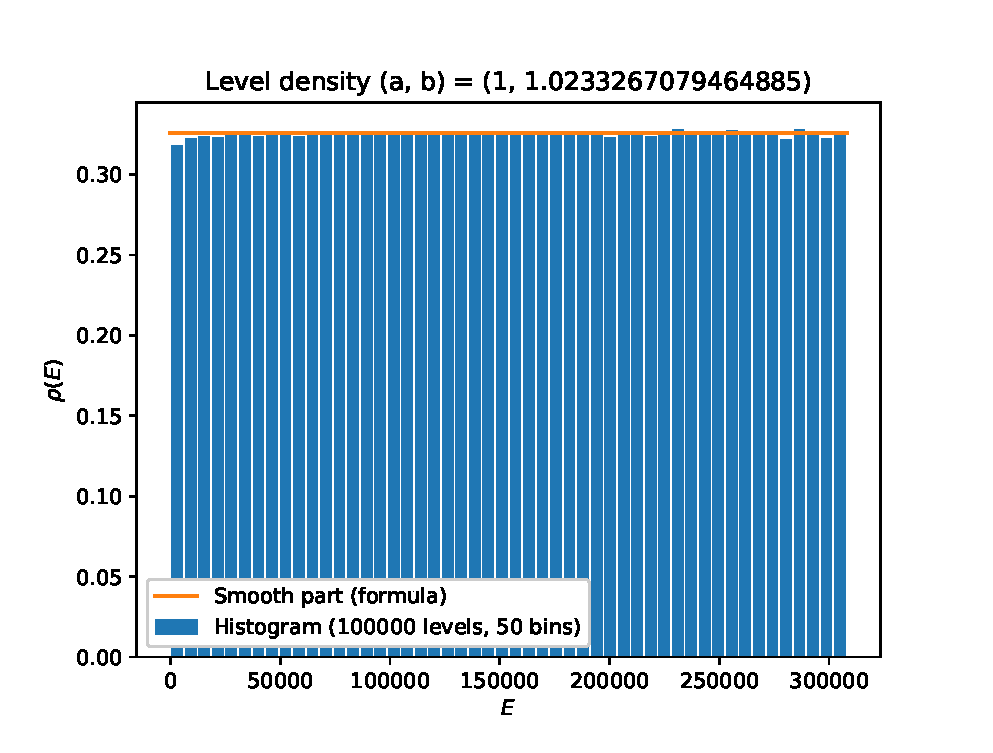
\epsfig{file=box2d_density.eps,width=\linewidth}
                \end{subfigure}
                \hfill
                \begin{subfigure}{0.49\linewidth}
                    \centering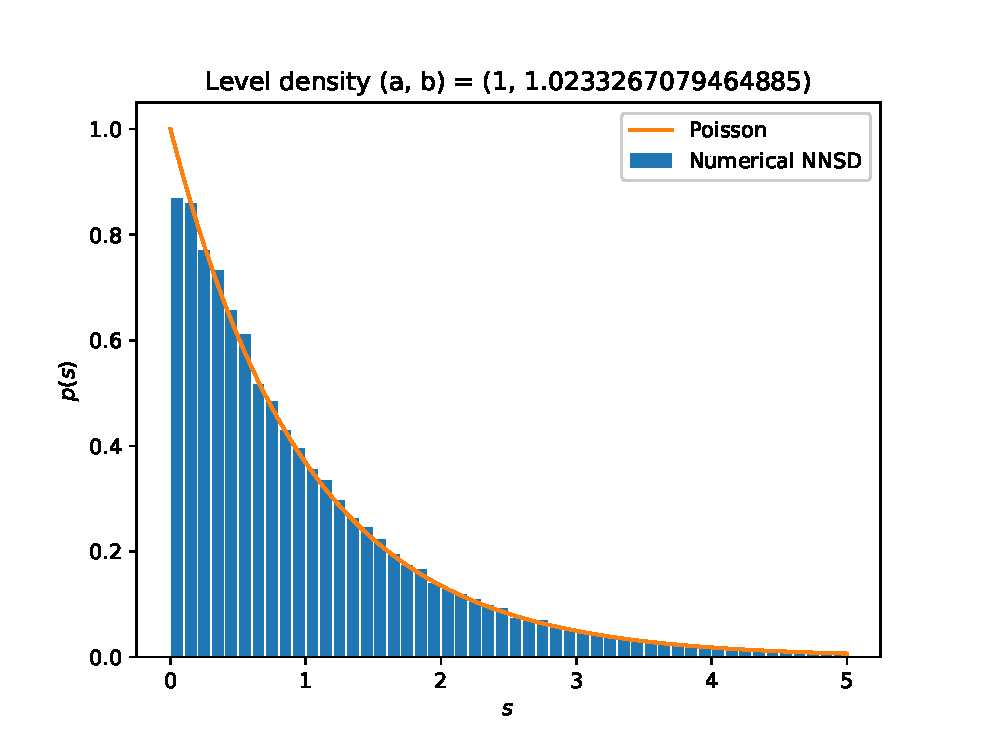
\epsfig{file=box2d_nnsd.eps,width=\linewidth}
                \end{subfigure}
                \begin{subfigure}{0.49\linewidth}
                    \centering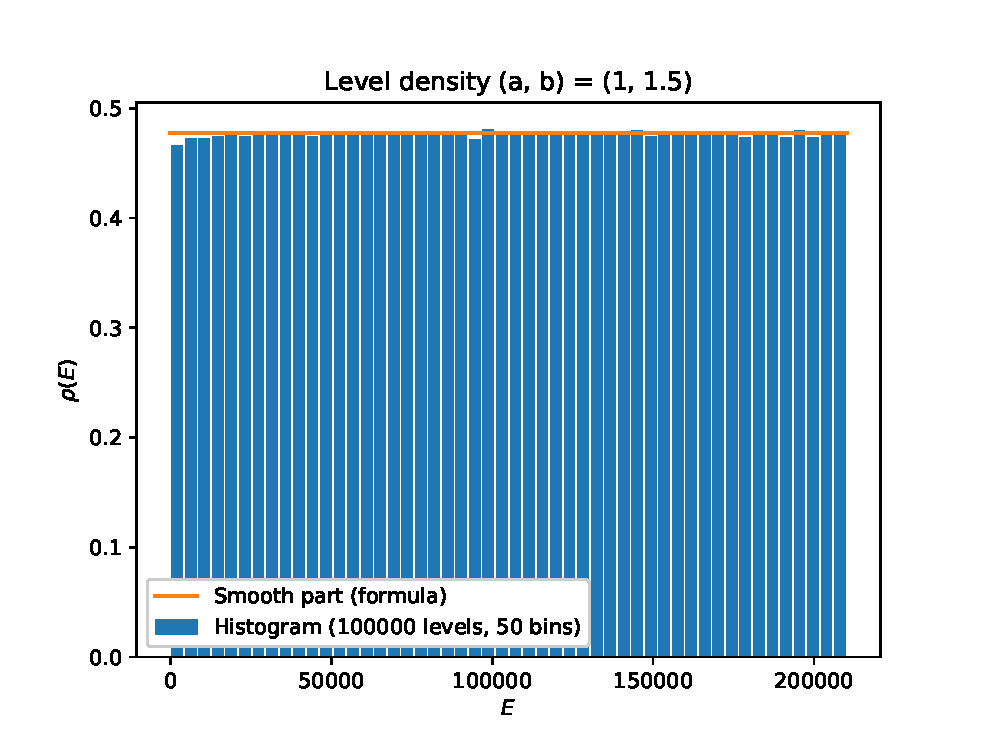
\epsfig{file=box2d_density_strong_resonance.eps,width=\linewidth}
                \end{subfigure}
                \hfill
                \begin{subfigure}{0.49\linewidth}
                    \centering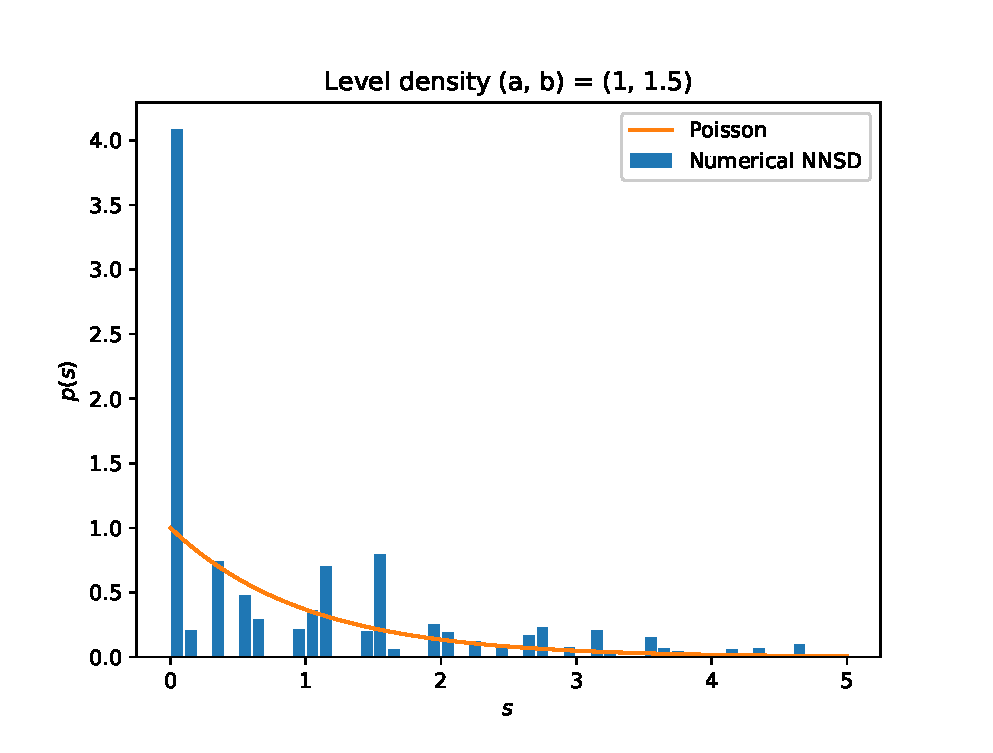
\epsfig{file=box2d_nnsd_strong_resonance.eps,width=\linewidth}
                \end{subfigure}
                \hfill
                \begin{subfigure}{0.98\linewidth}
                    \centering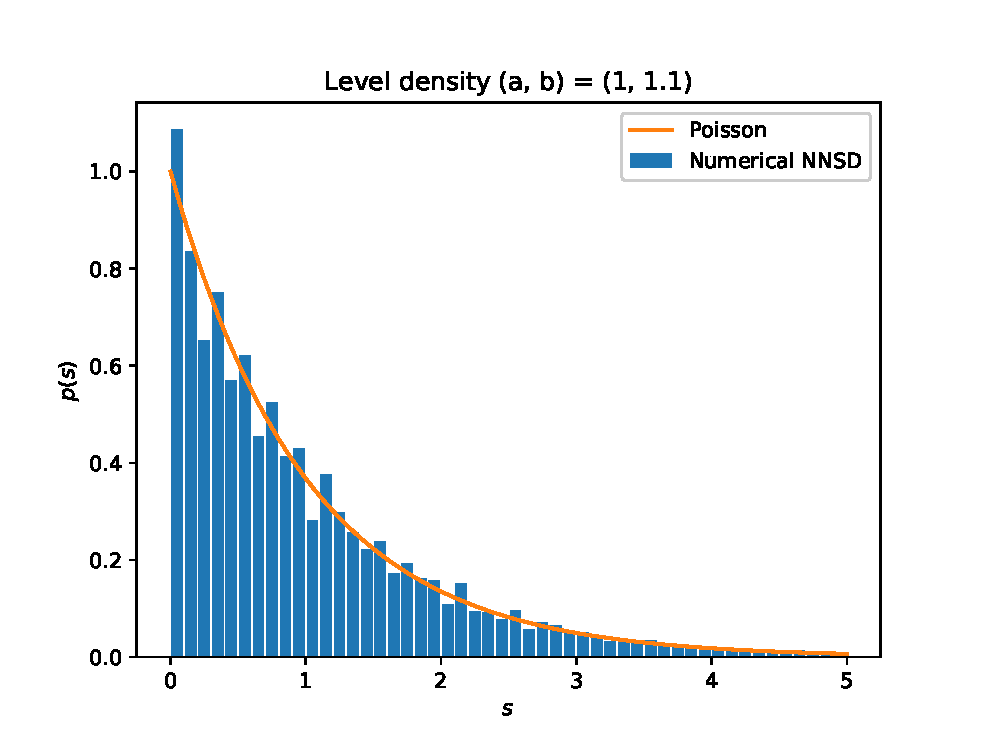
\epsfig{file=box2d_nnsd_weak_resonance.eps,width=0.5\linewidth}
                \end{subfigure}
                \hfill
                \caption{
                    \protect\small
                    Level density and nearest neighbour spacing distribution for the 2D rectangular infinite-well potential with $\hbar=M=1$ and (a) incommensurate lengths of the edges, (b) lengths in a strong resonance, and (c) lengths in a weak resonance.
                    The resonance introduces correlations among the levels.
                }	
                \label{fig:2Dbox}
            \end{figure}

        \end{solution}

\section{Chaotic systems}
    Here only a very brief overview of the history of quantum chaos is sketched.
    For more details I strongly recommend to read the first chapter of Mehta's monography~\cite{Meh04}.

    \subsection{Wigner surmise}\label{sec:Wigner}
        The field of quantum chaos started developing with the work of Eugene Wigner in 1950's. 
        At that time it was observed in the mesurements of high-lying slow nuclear resonances a lack of close states.
        At first it was being explained by imperfect measuring techniques, but then Wigner~\cite{Wig55} proposed and succeeded to use the Random Matrix Theory (RMT) to describe this suspicious behaviour of the resonances, and he formulated the so called
        \begin{theorem}
            {\bf (Wigner surmise)}
            Suppose we have a complicated and complex system with (often high) unknown number of degrees of freedom (such as a highly excited atomic nucleus\footnote{
                Low lying nuclear excitations are successfully explained by a plethora of models, \emph{e.g.} nuclear collective models, shell model, etc., with only a relatively small number of degrees of freedom.
                These models become more and more inacurate as the excitation energy increases, making the approximation of the complicated nucleon interactions impossible.})
            and we do not know anything about the interaction among the constituents.
            The only thing we know about the Hamiltonian is the symmetry it satisfies (rotational invariance, time-reversal invariance etc.).
            Then a sequence of consecutive energy levels with the same spin and parity will have the same statistical properties as the spectrum of a random matrix whose elements are independent numbers taken from the Gaussian normal distribution.
            Levels of different spin and parity are not correlated.\footnote{Spin and parity are conserved quantities (integrals of motion), and following the conclusions of Section~\ref{sec:Integrable} the must be uncorrelated.}
        \end{theorem}
        Soon after, Wigner derived the formula for the Nearest Neighbour Spacing Distribution of $2\times2$ random matrices invariant under rotations:
        \begin{equation}
            \label{eq:Wigner}
            p_{w}(s)=\frac{\pi}{2}s\e^{-\frac{\pi}{4}s^{2}},
        \end{equation}
        which is often called \remember{Wigner distribution}\footnote{Beware, there is another quantity in quantum mechanics called Wigner distribution (also called Wigner quasiprobability distribution or Wigner function).} (the derivation will be presented later in Sec.~\ref{sec:NNSD22}).

        Compared with the Poisson distribution for an integrable system~\eqref{eq:Poisson}, which has a maximum at $s=0$, \emph{i.e.} the levels tend to bunch together, the spectrum satisfying the Wigner distribution exhibits clear \remember{level repulsion} (the probability of coinciding levels is $p_{w}(0)=0$\footnote{This phenomenon is tightly related with the quantum no-crossing theorem.}). 

        \subsection{Bohigas conjecture}
        At the beginning the theory of quantum matrices served just as a tool to study statistical spectral properties of many-body systems under unknown interactions, whereas quantum counterparts of classically chaotic systems were studied by semiclassical methods in systems with only a few degrees of freedom.
        But then, in 1984, Bohigas, Giannoni and Schmit published a ground-breaking paper~\cite{Boh84} stating:
        \begin{theorem}
            {\bf (Bohigas (-Giannoni-Schmit) conjecture)}
            \remember{All quantum systems whose classical analogues are chaotic exhibit the same spectral fluctuation properties as predicted by the theory of random matrices.}
            On the contrary, quantum systems whose classical analogues are stable (not necessarily integrable) have uncorrelated energy levels.
        \end{theorem}
        This paper established the field that is since then called quantum chaos.

        Now some remarks: 
        \begin{enumerate}
            \item Until now the conjecture has not been proved in its generality.\footnote{
                    There are several different classes of classically chaotic systems:
                    \begin{equation*}
                        \boxed{\text{Ergodic}}
                            \supset\boxed{\text{Weakly Mixing (WM)}}
                            \supset\boxed{\text{Strongly Mixing (SM)}}
                            \supset\boxed{\text{Kolmogorov ($K$-)}}
                            \supset\boxed{\text{Bernoulli ($B$-)}}
                    \end{equation*}
                    The complete discussion of this classification is beyond the scope of this lecture (and it belongs to the area of classical chaos theory), you can find it in~\cite{Sin77}.
                    It has been proved, though, that mixing at the classical level is sufficient to generate random matrix statistics.
                } 
                However, there is vast list of numerical studies based on a wide variety of systems that support its validity (but there are also several counter-examples of systems that are classically regular, but have random-matrix-like quantum spectrum\footnote{For example the Šeba's billiard: a circular billiard with a $\delta$-function sitting in the middle.} and vice versa).
        \end{enumerate}

\section{Gaussian random matrix ensembles}
    The main question is the following: 
    What are some significant properties of an ensemble of matrices whose elements are random variables with a specific probability law? 
    What can we say about correlations among the eigenlevels and eigenvectors?
    
    As happens many theories, their pioneers are often forgotten and hardly mentioned. 
    A developement of the random matrix theory began in 1920s~\cite{Wis28} but did not draw much attention at that time.
    The theory became more popular when Wigner formulated his surmise, see Section~\ref{sec:Wigner},
    but a mathematically rigorous foundations of the so called Random Matrix Theory (RMT) were established in a series of beautiful papers by Dyson~\cite{Dys62}\footnote{
        Freeman John Dyson, who recently passed away, was an author or co-author of many seminal ideas and theorems in mathematics and physics, although only a few are named after him, probably due to his modesty (the most famous is the Dyson series, leading to Feynman-Dyson diagrams). As a curiosity, he became a professor without having finished his Ph.D. studies.
        He is a laureate of the Templeton Prize.
    }
    (the distribution~\ref{eq:Wigner} is sometimes called \emph{Wigner-Dyson distribution}).
    He introduced the classification of the Gaussian random matrix ensembles according to their invariance properties under time reversal and proved that there are only three classes of them (universality classes) and he aptly stated: ``What is here requiered is a new kind of statistical mechanics, in which we renounce exact knowledge not of the state of the system but of the system itself.
    We picture a complex nucleus as a `black box' in which a large number of particles are interacting acording to unknown laws.
    The problem then is to define in a mathematically precise way an ensemble of systems in which all possible laws of interaction are equally possible.''

    So what is the Gaussian random matrix and what are the available ensembles?
    \begin{theorem}\label{th:GE}
        The Gaussian random matrix $\matrix{H}$ is a matrix from an ensemble of matrices with probability distribution $P(\matrix{H})$, satisfying
        \begin{enumerate}
            \item The probability distribution is invariant under a given transformation $\matrix{W}$,
                \begin{equation}
                    P(\matrix{H})=P(\matrix{H}'),\quad\text{where}\ \matrix{H'}=\matrix{W}^{-1}\matrix{H}\matrix{W}
                \end{equation}
                (necessary if we want matrix $\matrix{H}$ to correspond with the Hamiltonian of a physical system).
            \item Matrix elements of $\matrix{H}$ are statistically independent.
        \end{enumerate}
        From these two requirements it follows that the distribution of matrix elements is Gaussian (this statement will be proved in Section~\ref{sec:NNSD22}).
    \end{theorem}

    The three available ensembles are\footnote{
        From a mathematical point of view, these three classes exhaust the distinct real commutative normed division algebras (in effect number systems).
        That is why there are just these three ensembles.
    }: 
    \begin{enumerate}
        \item {\bf Gaussian Orthogonal Ensemble ($\ensemble{GOE}$), $\beta=1$}: 
            Time-reversal invariant systems with $\operator{T}^{2}=1$.
            This ensemble is invariant under orthogonal transformation,
            \begin{equation}\label{eq:PHInvariance}
                P(\matrix{H})=P\left(\transpose{\matrix{O}}\matrix{H}\matrix{O}\right),
                \quad\transpose{\matrix{O}}\matrix{O}=\matrix{1}.
            \end{equation}
            The matrix $\matrix{H}$ modelling the Hamiltonian of our system is real symmetric and has $N(N+1)/2$ independent real components.
            The majority of systems belongs to the $\ensemble{GOE}$.

        \item {\bf Gaussian Unitary Ensemble ($\ensemble{GUE}$), $\beta=2$}: 
            System not invariant under time reversal.
            This ensemble is invariant under unitary transformation,
            \begin{equation}
                P(\matrix{H})=P\left(\matrix{U}^{-1}\matrix{H}\matrix{U}\right),
                \quad\matrix{U}^{-1}\matrix{U}=\matrix{1}.
            \end{equation}
            The matrix $\matrix{H}$ is complex Hermitian and has $N^{2}$ independent real components.
            $\ensemble{GUE}$ is suitable, \emph{e.g.}, for systems in external magnetic field.
        
        \item {\bf Gaussian Symplectic Ensemble ($\ensemble{GSE}$), $\beta=4$}:
            Time-reversal invariant systems with $\operator{T}^{2}=-1$.
            This ensemble is invariant under symplectic transformation,
            \begin{equation}
                P(\matrix{H})=P\left(\matrix{S}^{-1}\matrix{H}\matrix{S}\right),
                \quad\matrix{S}^{-1}\matrix{H}\matrix{S}=\matrix{1}.
            \end{equation}
            The matrix $\matrix{H}$ is quaternionic Hermitian and has $N(2N-1)$ independent components.\footnote{Quaternionic $N\times N$ matrix can be modelled by $2N\times 2N$ complex matrices.}
            This is the least common case to encounter.
            Systems in this class exhibit Kramers degeneracy.
            Systems with half-integer spins belong to this class. 
    \end{enumerate} 
    The index $\beta$ is called \remember{Dyson number}.
    Examples of spectra of matrices belonging to these three ensembles are given in Figure~\ref{fig:Ensembles}(a). 

    \subsection{Other ensembles}
    If we weaken any of the conditions of Theorem~\ref{th:GE}, we may extend the number of universality classes and introduce new ensembles:
    \begin{itemize}
        \item Altland-Zirnbauer universality classes~\cite{Alt97} (7 additional classes by relaxing Equation~\eqref{eq:PHInvariance}, taking into account particle-hole symmetry or chiral symmetry).
        \item Random unitary matrices (Gaussian Circular Ensembles) for modelling the scattering $S$-matrix instead of Hamiltonian matrix.
        \item Random band matrices.
        \item Ginibre ensembles~\cite{Gin65} (condition~\eqref{eq:PHInvariance} completely disregarded).
    \end{itemize} 
    In these notes we shall restrict ourselves on the Gaussian ensembles only.

    \subsection{$2\times2$ GOE matrices}\label{sec:NNSD22}
        Many of the properties of random matrix ensembles can be demonstrated on the smallest nontrivial matrices possible (and some of the properties can be explicitly derived only for these matrices).

        \subsubsection{Probability distribution}
            In this section we will derive the properties of a $2\times2$ random matrix from the Gaussian Orthogonal Ensemble (usually abreviated as $\ensemble{GOE}$ random matrix).
            We will follow the requirements given in Theorem~\ref{th:GE}.

            The matrix $\matrix{H}\in\ensemble{GOE}(2)$ is real and symmetric, so it has only three independ elements $H_{11},H_{22},H_{12}$.
            The probability is normalized,
            \begin{equation}\label{eq:Hnorm}
                \int\d H_{11}\d H_{12}\d H_{22}P(\matrix{H})=1
            \end{equation}

            1. The probability distribution has to be invariant under orthogonal transformation,
            \begin{equation}\label{eq:OHO}
                P(\matrix{H})=P(\matrix{H}'),\qquad\text{where}\quad\matrix{H}'=\transpose{\matrix{O}}\matrix{H}\matrix{O},
            \end{equation}
            where a general $2\times2$ orthogonal matrix can be written as
            \begin{align}\label{eq:O}
                \matrix{O}(\theta)
                    &=\makematrix{\cos\theta & \sin\theta \\ -\sin\theta & \cos\theta}
                    \approx\makematrix{1 & \theta \\ -\theta & 1}\\
                    \transpose{\matrix{O}}(\theta),
                    =\matrix{O}^{-1}(\theta)
                    &=\makematrix{\cos\theta & -\sin\theta \\ \sin\theta & \cos\theta}
                    \approx\makematrix{1 & -\theta \\ \theta & 1}
            \end{align}
            and depends on just one parameter (angle) $\theta$.
            Without the loss of generality, we can consider infinitesimal rotations $\theta\approx0$ only.
            Then it follows from~\eqref{eq:OHO} that
            \begin{align}
                \makematrix{H'_{11} & H'_{12} \\ H'_{21} & H'_{22}}
                    &=\makematrix{1 & -\theta \\ \theta & 1}
                        \makematrix{H_{11} & H_{12} \\ H_{21} & H_{22}}
                        \makematrix{1 & \theta \\ -\theta & 1}\nonumber\\
                    &=\makematrix{H_{11}-2\theta H_{12}+\theta^{2}H_{22} & 
                        \theta H_{11}+H_{12}-\theta^{2}H_{12}-\theta H_{22} \\
                        \theta H_{11}-\theta^{2}H_{12}+H_{12}-\theta H_{22} & 
                        \theta^{2}H_{11}+2\theta H_{12}+H_{22}}\nonumber\\
                    \label{eq:HpH}
                    &\approx\makematrix{H_{11}-2\theta H_{12} & H_{12}+\theta\left(H_{11}-H_{22}\right) \\
                        H_{12}+\theta\left(H_{11}-H_{22}\right) & H_{22}+2\theta H_{12}}
            \end{align}
            (up to the $1^{\text{st}}$ order in $\theta$).

            2. The matrix elements are statistically independent, which means that the probability $P(\matrix{H})$ is given by the product of probabilities of individual elements, 
            \begin{equation}
                P(\matrix{H})
                    =P_{11}(H_{11})P_{12}(H_{12})P_{22}(H_{22}).
            \end{equation}
            Substituting from~\eqref{eq:OHO} and~\eqref{eq:HpH} we get 
            \begin{align}
                P(\matrix{H})
                    &=P_{11}(H'_{11})P_{12}(H'_{12})P_{22}(H'_{22})\nonumber\\
                    &=P_{11}\left(H_{11}-2\theta H_{12}\right)
                        P_{12}\left(H_{12}+\theta(H_{11}-H_{22})\right)
                        P_{22}\left(H_{22}+2\theta H_{12}\right)\nonumber\\
                    &\equationcomment{\text{$1^{\text{st}}$ order Taylor expansion}}\nonumber\\
                    &\approx \left[P_{11}(H_{11})-2\theta H_{12}\derivative{P_{11}}{H_{11}}\right]
                        \left[P_{12}(H_{12})+\theta(H_{11}-H_{22})\derivative{P_{12}}{H_{12}}\right]
                        \left[P_{22}(H_{22})+2\theta H_{12}\derivative{P_{22}}{H_{22}}\right]\nonumber\\
                    &=P(\matrix{H})\left\{
                        \left[1-2\theta\frac{H_{12}}{P_{11}}\derivative{P_{11}}{H_{11}}\right]
                        \left[1+\theta\frac{H_{11}-H_{22}}{P_{12}}\derivative{P_{12}}{H_{12}}\right]
                        \left[1+2\theta\frac{H_{12}}{P_{22}}\derivative{P_{22}}{H_{22}}\right]
                        \right\}\nonumber\\
                    &\equationcomment{\text{$1^{\text{st}}$ order terms in $\theta$}}\nonumber\\
                    &\approx P(\matrix{H})\left\{1-\theta\left[
                        2\frac{H_{12}}{P_{11}}\derivative{P_{11}}{H_{11}}
                        -2\frac{H_{12}}{P_{22}}\derivative{P_{22}}{H_{22}}
                        -\frac{H_{11}-H_{22}}{P_{12}}\derivative{P_{12}}{H_{12}}
                        \right]\right\}.
            \end{align}
            The last expression has to be invariant with respect to $\theta$, so the bracket must vanish:
            \begin{equation}
                2\frac{H_{12}}{P_{11}}\derivative{P_{11}}{H_{11}}
                -2\frac{H_{12}}{P_{22}}\derivative{P_{22}}{H_{22}}
                -\frac{H_{11}-H_{22}}{P_{12}}\derivative{P_{12}}{H_{12}}=0
            \end{equation}
            \begin{equation}
                \frac{1}{P_{12}H_{12}}\derivative{P_{12}}{H_{12}}-\frac{2}{H_{11}-H_{22}}
                \left(\frac{1}{P_{11}}\derivative{P_{11}}{H_{11}}-\frac{1}{P_{22}}\derivative{P_{22}}{H_{22}}\right)=0
            \end{equation}
            We obtain an equation for the distributions $P_{11}$, $P_{12}$, $P_{22}$, which can be separated into two independent equations,
            \begin{align}
                \frac{1}{P_{12}H_{12}}\derivative{P_{12}}{H_{12}}
                    &=-4A\nonumber\\
                \left(\frac{1}{P_{11}}\derivative{P_{11}}{H_{11}}-\frac{1}{P_{22}}\derivative{P_{22}}{H_{22}}\right)
                    &=-2A\left(H_{11}-H_{22}\right)
            \end{align}
            (we called the arbitrary separation constant $-4A$).
            The second equation can be further separated into
            \begin{align}
                \derivative{P_{11}}{H_{11}}+2AH_{11}&=-B\nonumber\\
                \derivative{P_{22}}{H_{22}}+2AH_{22}&=-B.
            \end{align}
            The solutions of the separated $1^{\text{st}}$ differential equations are
            \begin{align}
                P_{12}&=C_{12}\e^{-2AH_{12}^{2}},\nonumber\\
                P_{11}&=C_{11}\e^{-AH_{11}^{2}-BH_{11}},\\
                P_{22}&=C_{22}\e^{-AH_{22}^{2}-BH_{22}},
            \end{align}
            where $C_{11}$, $C_{12}$, and $C_{22}$ are integration constant.

            The probability distribution is therefore
            \begin{equation}
                \label{eq:PHelements}
                P(\matrix{H})=C\e^{-A\left(H_{11}^{2}+H_{22}^{2}+2H_{12}^{2}\right)-B\left(H_{11}+H_{22}\right)},
            \end{equation}
            where $C=C_{11}C_{12}C_{22}$ is a normalization constant constrained by condition~\eqref{eq:Hnorm}, $A$ fixes the unit of energy, and $B$ gives the shift of energy (can be made $0$ by an appropriate choice of zero energy), so the distribution can be finally written in the form
            \begin{equation}
                \label{eq:PH}
                \important{P(\matrix{M})=C\e^{-A\trace\matrix{H}^{2}}}.
            \end{equation}

            A couple of observations and comments:
            \begin{enumerate}
                \item 
                    From the distribution~\eqref{eq:PHelements} it follows that the nondiagonal elements have half the dispersion that the diagonal elements.
                    This is important for numerical generation of $\ensemble{GOE}$ random matrices.

                \item
                    The expression~\eqref{eq:PH} is valid for other Gaussian matrix ensembles ($\ensemble{GUE}$ and $\ensemble{GSE}$) and for an arbitrary matrix dimension $N$).    
            \end{enumerate}

        \subsubsection{Eigenvalues distribution}
            Here we want to move from the matrix element probability distribution~\eqref{eq:PH} to the probability distribution of finding a particular pair of eigenvalues (for a $N=2$ matrix).
            The eigenvalues of the $2\times2$ matrix are
            \begin{equation}
                E_{\pm}=\frac{1}{2}\left(H_{11}+H_{22}\right)\pm\frac{1}{2}\sqrt{\left(H_{11}-H_{22}\right)^{2}+4H_{12}^{2}}.
            \end{equation}
            The original matrix is then
            \begin{equation}
                \matrix{H}=\transpose{\matrix{O}}\diagonal{E_{+},E_{-}}\matrix{O},
            \end{equation}
            where the eigenvectors matrix $\matrix{O}$ is the orthogonal transformation matrix~\eqref{eq:O}.
            Substitution gives
            \begin{align}
                H_{11}&=E_{+}\cos^{2}\theta+E_{-}\sin^{2}\theta\nonumber\\
                H_{22}&=E_{+}\sin^{2}\theta+E_{-}\cos^{2}\theta\\
                H_{12}&=\left(E_{+}-E_{-}\right)\sin\theta\cos\theta.\nonumber
            \end{align}
            This specifies the transformation $\left(E_{+},E_{-},\theta\right)\leftrightarrow\left(H_{11},H_{22},H_{12}\right)$ whose Jacobian is
            \begin{align}
                J&=\det\partialderivative{\left(H_{11},H_{22},H_{12}\right)}{\left(E_{+},E_{-},\theta\right)}\nonumber\\
                    &=\det\makematrix{\cos^{2}\theta & \sin^{2}\theta & -2(E_{+}-E_{-})\sin\theta\cos\theta \\
                        \sin^{2}\theta & \cos^{2}\theta & 2(E_{+}-E_{-})\sin\theta\cos\theta \\
                        \sin\theta\cos\theta & -\sin\theta\cos\theta & (E_{+}-E_{-})\left(\cos^{2}\theta-\sin^{2}\theta\right)}\nonumber\\
                    &=\left(E_{+}-E_{-}\right)\left[cos^{4}\theta\left(\cos^{2}\theta-\sin^{2}\theta\right)+2\sin^{4}\theta\cos^{2}\theta+2\sin^{4}\theta\cos^{2}\theta\right.\nonumber\\
                    &\qquad\left.+2\sin^{2}\theta\cos^{4}\theta+2\sin^{2}\theta\cos^{4}\theta-\sin^{4}\theta\left(\cos^{2}\theta-\sin^{2}\theta\right)\right]\nonumber\\
                    &=\left(E_{+}-E_{-}\right)\left[cos^{4}\theta\cos2\theta+\sin^{2}2\theta-\sin^{4}\theta\cos2\theta\right]\nonumber\\
                    &=\left(E_{+}-E_{-}\right)\left[\left(cos^{2}\theta+\sin^{2}\theta\right)\left(cos^{2}\theta-\sin^{2}\theta\right)\cos2\theta+\sin^{2}2\theta\right]\nonumber\\
                    &=\left(E_{+}-E_{-}\right)\left[\cos^{2}2\theta+\sin^{2}2\theta\right]\nonumber\\
                    &=E_{+}-E_{-},
            \end{align}
            so the desired (joint) probability density is
            \begin{align}
                P\left(E_{+},E_{-}\right)
                    &=\left. P(H_{11},H_{22},H_{12})\right|
                        _{\left(H_{11},H_{22},H_{12}\right)\mapsto{\left(E_{+},E_{-},\theta\right)}}\nonumber\\
                    &=C\abs{J}\e^{-A\trace{\matrix{H}^{2}}}\nonumber\\
                    \label{eq:PE2}
                    &=C\abs{E_{+}-E_{-}}\e^{-A\left(E_{+}^{2}+E_{-}^{2}\right)}.
            \end{align}

            Some comments:
            \begin{enumerate}
                \item The eigenvalues distribution is independent of the angle $\theta$.
                \item For a general $N$-dimensinal matrix from a Gaussian ensemble with Dyson index $\beta$, the joint probability distribution for eigenvalues is
                    \begin{equation}
                        \label{eq:PE}
                        P(E_{1},\dotsc,P_{N})=C\prod_{j<k}^{1\dotsb N}\abs{E_{j}-E_{k}}^{\beta}\e^{-A\sum_{j=1}^{N}E_{j}^{2}}.
                    \end{equation}
            \end{enumerate}

        \subsubsection{Nearest neighbour spacing distribution}
            NNSD is obtained from~\eqref{eq:PE2} via
            \begin{align}
                p(s)&=\intinf\d E_{+}\intinf\d E_{-}\,\delta\left(s-\abs{E_{+}-E_{-}}\right)P(E_{+},E_{-})\nonumber\\
                    &=C\intinf\d E_{+}\intinf\d E_{-}\,\delta\left(s-\abs{E_{+}-E_{-}}\right)\abs{E_{+}-E_{-}}\e^{-A\left(E_{+}^{2}+E_{-}^{2}\right)}\nonumber\\
                    &\equationcomment{\text{We suppose that $E_{+}>E_{-}$ and substitute $E_{+}\rightarrow\sigma$:} \\
                        \sigma=E_{+}-E_{-},\\
                        \d\sigma=\d E_{+}}\nonumber\\
                    &=C\intinf\d E_{-}\,s\e^{-A\left(s^{2}+2sE_{-}+2E_{-}^{2}\right)}\nonumber\\
                    &=Ds\e^{-\frac{A}{2}s^{2}}.
            \end{align} 
            After normalizing and rescaling to have a unit mean level spacing~\eqref{eq:psnorm}, we land to the already discussed Wigner distribution~\eqref{eq:Wigner},
            \begin{equation}\label{eq:Wigner1}
                p_{w}(s)=\frac{\pi}{2}\,s\e^{-\frac{\pi}{4}s^{2}}.
            \end{equation}

            \begin{figure}[!htbp]
                \begin{subfigure}{0.55\linewidth}
                    \centering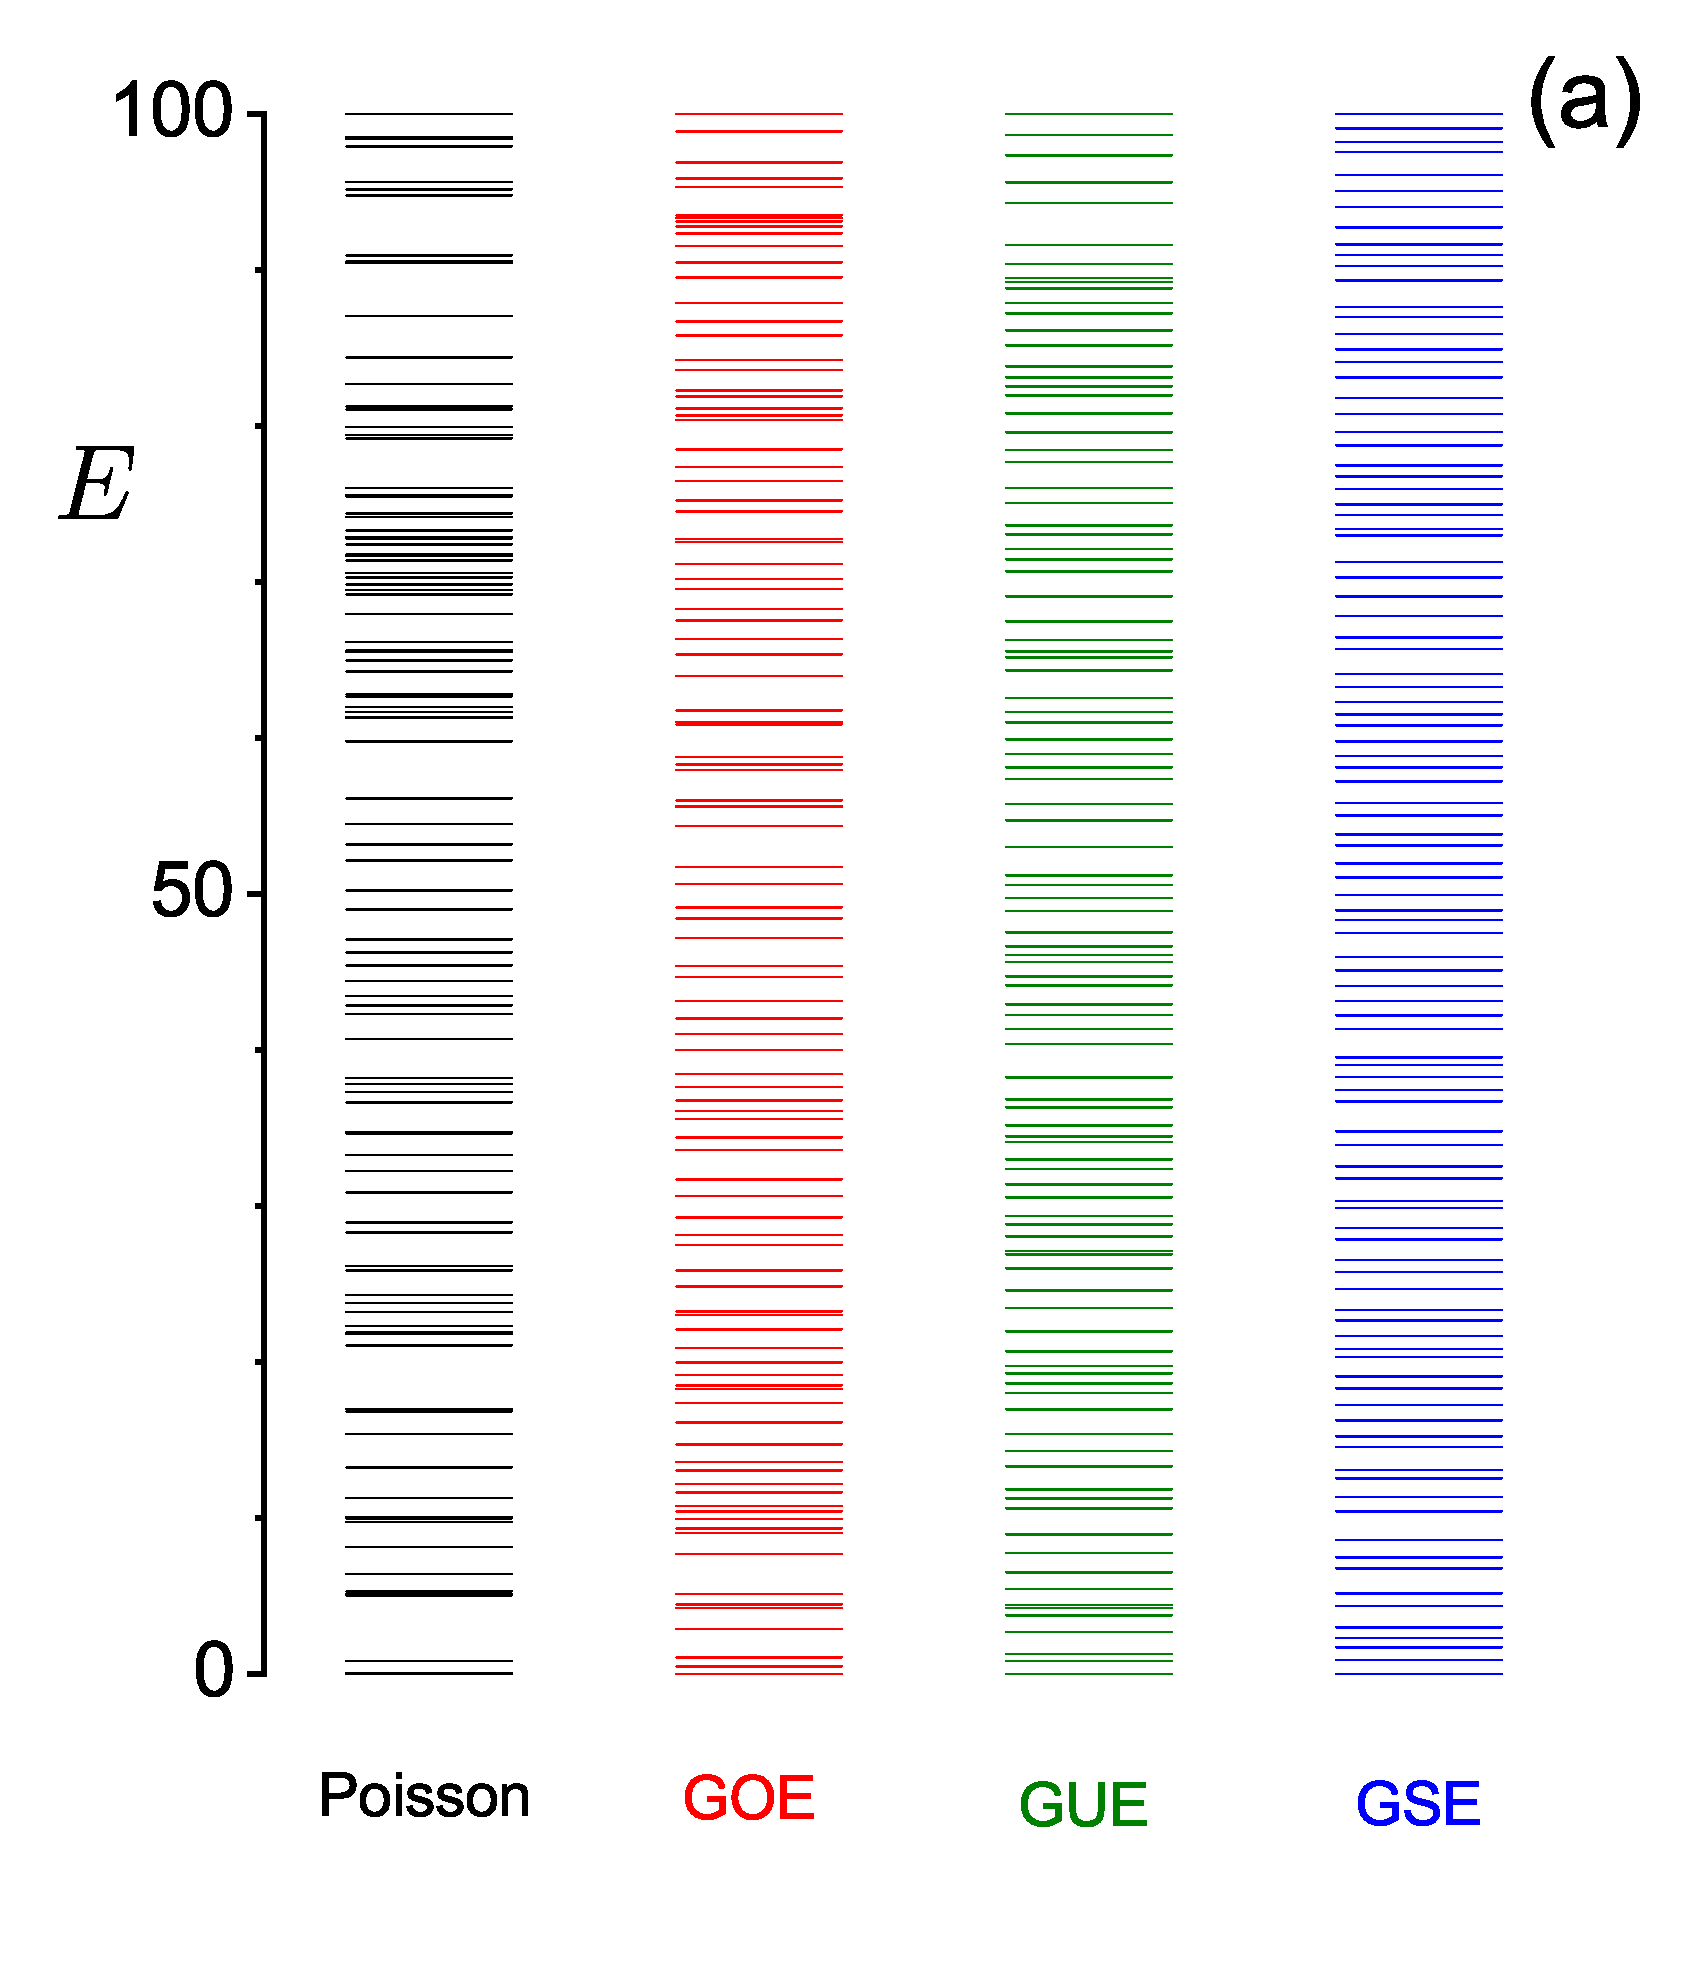
\epsfig{file=ensembles.eps,width=\linewidth}
                \end{subfigure}
                \hfill
                \begin{subfigure}{0.44\linewidth}
                    \centering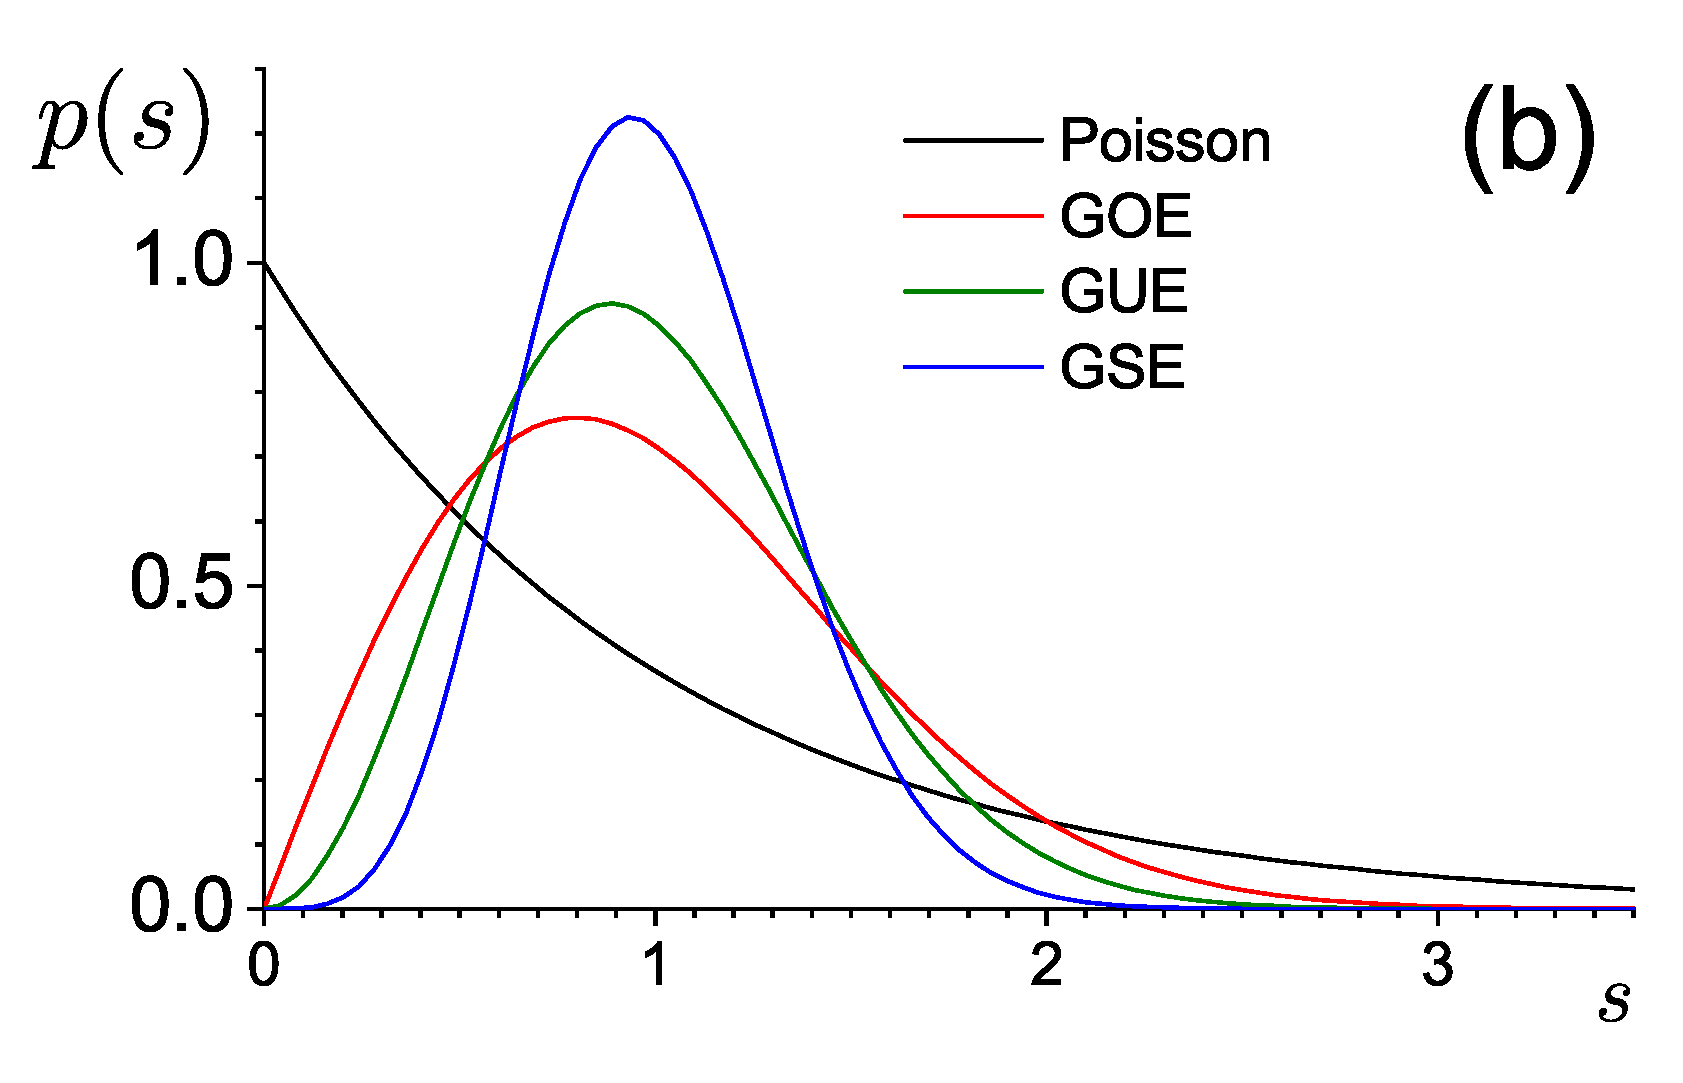
\epsfig{file=nnsd.eps,width=\linewidth}
                    \centering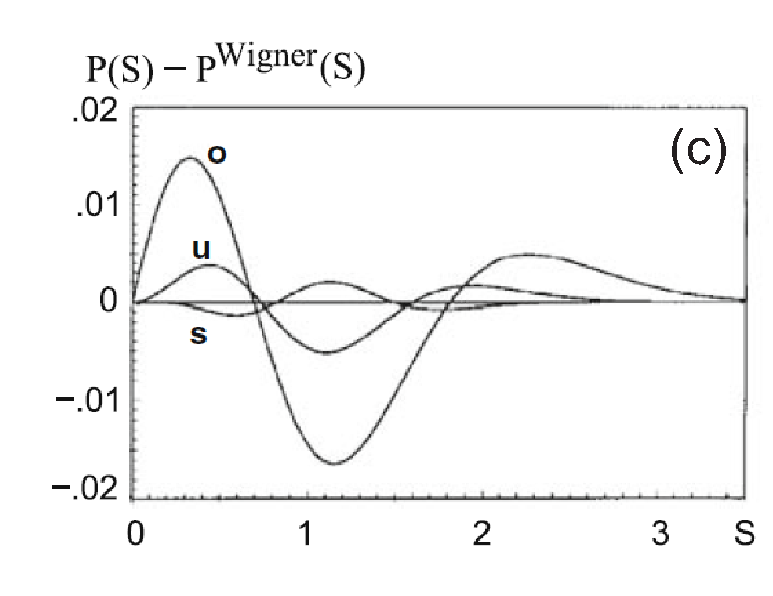
\epsfig{file=psdiff.eps,width=\linewidth}
                \end{subfigure}
                \caption{
                    \protect\small
                    (a) Example of spectra with different NNSD.
                    The spectra are normalized to $\langle s\rangle=1$.
                    The stronger the level repulsion given by the Dyson number,
                    the more uniform looks the spectrum.
                    For levels with Poisson distribution there are both bunches of levels and wide gaps.
                    (b) Probability distributions~\eqref{eq:WignerAll} corresponding to chaotic systems compared with the Poisson distribution~\eqref{eq:Poisson} corresponding to an integrable system.
                    (c) Absolute deviation of $p_{w}(s)$ for $2\times2$ matrices from the NNSD for infinite-size matrices.
                    The largest deviation is observed for $\ensemble{GOE}$ at $s\approx0.4$.
                    However, the deviation does not exceed $4\%$.
                    This panel is taken from~\cite{Haa10}.
                }	
                \label{fig:Ensembles}
            \end{figure}

            Comments:
            \begin{enumerate}
                \item Distribution~\eqref{eq:Wigner1} is valid for matrices $2\times2$ only.
                    For higher-dimensional matrices it is impossible to get a closed formula for the spacing density, it can be found only numerically.
                    However, the deviation from $p_{w}$ is at most in the order of a few per cent, even when $N\rightarrow\infty$, see Figure~\ref{fig:Ensembles}(c).
                    For practical purposes the distribution~\eqref{eq:Wigner1} is good enough, and is widely used for matrices of an arbitrary dimension.

                \item Similar formulae can be derived for other ensembles.
                    Normalized NNSD for all three ensembles of Gaussian matrices are
                    \begin{align}
                        &\ensemble{GOE}:
                        &p_{w}^{(\beta=1)}(s)
                            &=\frac{\pi}{2}\,s\e^{-\frac{\pi}{4}s^{2}}\nonumber\\
                        \label{eq:WignerAll}
                        &\ensemble{GUE}:
                        &p_{w}^{(\beta=2)}(s)
                            &=\frac{32}{\pi^{2}}\,s^{2}\e^{-\frac{4}{\pi}s^{2}}\\
                        &\ensemble{GSE}:
                        &p_{w}^{(\beta=4)}(s)
                            &=\left(\frac{64}{9\pi}\right)^{3}s^{4}\e^{-\frac{64}{9\pi}s^{2}}\nonumber
                    \end{align}
                    and they are displayed in Figure~\ref{fig:Ensembles}(b).
                    An important observation is that the strength of the repulsion depends on the Dyson number,
                    \begin{equation}
                        p_{w}^{(\beta)}\approx s^{\beta}\quad\text{for}\ s\ll1.
                    \end{equation} 
            \end{enumerate}

    \subsection{Wigner semicircle law}
        A final remark related to the spectra of random matrices is the average level density.
        It is given by integral
        \begin{equation}
            \overline{\rho}(E)=\int\d E_{2}\dotsb\d E_{N}P(E,E_{2},\dotsc,E_{N}),
        \end{equation}
        where $P$ is the joint probability density~\eqref{eq:PE}.
        
        When matrix dimension $N$ is high, $N\rightarrow\infty$, the integral\footnote{
            This integral requires a rather advanced mathematical tools.
            The most straighforward way to perform it is via Grassmann integration.
        }
        converges to the \remember{Wigner semicircle law}~\cite{Wig57}
        \begin{equation}
            \label{eq:Semicircle}
            \boxed{
                \overline{\rho}(E)=\left\{\begin{array}{ll}
                    \frac{1}{2\pi}\sqrt{1-E^{2}} & \abs{E}\leq 1,\\
                    0 & \abs{E}>1,
                \end{array}
                \right.
            }
        \end{equation}
        where, in order to secure convergence of the integral, we impose the following condition,
        \begin{equation}
            \label{eq:SemicircleCondition}
            \overline{H_{jk}H_{kj}}=\overline{H_{jj}^{2}}=\frac{1}{4N}.
        \end{equation}
        If we go back to~\eqref{eq:PH}, we see that the variance $\sigma^{2}$ of matrix elements is related with $A$ via
        \begin{equation}
            A=\frac{1}{2\sigma^{2}}.
        \end{equation}
        Hence condition~\eqref{eq:SemicircleCondition} is satisfied if
        \begin{equation}
            \sigma=\frac{1}{2\sqrt{N}}.
        \end{equation}
        
        Comments:
        \begin{itemize}
            \item 
                The semicircle law~\eqref{eq:Semicircle} is valid in the limit $N\rightarrow\infty$ only.
                For smaller matrix sizes, the behaviour of the level distribution at $E=\pm1$ is not abrupt (\emph{i.e.}, changing from $\overline{\rho}=0$ to $\overline{\rho}>0$ with an infinite jump in the derivative $\overline{\rho}'$), but smooth.
                Even though for large matrices these finite-size effect are rather tiny, they must be taken into account in the unfolding process discussed in Section~\ref{sec:Unfolding}.

            \item The semicircle law is valid also for $\ensemble{GUE}$ and $\ensemble{GSE}$. 
        
            \item 
                For practical numerical purposes, the level density $\overline{\rho}(E)$ is approximated by a histogram.
                In a real system given by one particular Hamiltonian, we have just one spectrum, therefore it is necessary to have the highest number of converging levels possible in order to get a resonably precise approximation of $\overline{\rho}(E)$.
                On the other hand, random matrices are taken from the ensemble, so one can calculate an ensemble average of all the matrix properties, including the level density $\overline{\rho}(E)$.
                This means that it is possible to define (and calculate) properties of very small random matrices, which however, does not make sense for real systems.\footnote{
                    For example the level density of $\ensemble{GOE}$ matrix $1\times1$ is just a Gaussian function~\eqref{eq:PH}.
                }

            \item 
                While the fluctuation properties, such as the NNSD, has a universal validity, the semicircle law of level density is a specific property of the Gaussian matrix ensembles.
                More about it in the following section.
        \end{itemize}

    \subsection{Generating a $\ensemble{GOE}$ matrix}
        A matrix from the Gaussian matrix ensembles can be generated numerically by using the distribution~\eqref{eq:PH}.
        Namely, a $\ensemble{GOE}$ matrix is a symmetric matrix whose elements are normally distributed values with variance $\sigma^{2}$ of the non-diagonal items and $2\sigma^{2}$ for the diagonal items:
        \begin{equation}
            H_{jk}=H_{kj}=N\left(0,(1+\delta_{jk})\sigma^{2}\right),
        \end{equation}
        where $\delta_{kj}$ is the Kronecker delta. 

    \begin{task}\label{task:GOE}
        Make a routine to generate a $\ensemble{GOE}$ matrix and calculate its eigenvalues.
        Show that for sufficiently large matrices, $N\gtrapprox1000$,\footnote{
            Standard routines based on LAPACK library can diagonalize matrices up to $N\approx20000$ in a PC with 16 GB RAM.
            However, since the computational complexity of the diagonalization algorithm is $\mathcal{O}(N^{3})$, it takes enormous time to diagonalise such large matrices (usually several hours), while matrices of $N\approx1000$ are usually calculated within seconds.
        }
        the level density is very well approximated by the Wigner semicircle law.
        In order to get more precise estimate of the level density, calculate an average over a sample of several random matrices.
    \end{task}

\section{Statistical analysis of a quantum spectrum}
    In this section it will be assumed that we have spectrum of a general quantum system, and our goal is to prepare the spectrum in such a way that we could use spectral statistics to distinguish whether the levels are correlated or not.

    \subsection{Level density}
        The level density can always be written as a sum of two parts: the smooth part $\overline{\rho}(E)$ and the oscillatory part~$\tilde{\rho}(E)$,
        \begin{equation}
            \rho(E)\equiv\overline{\rho}(E)+\tilde{\rho}(E).
        \end{equation}  
        The smooth part gives an average number of levels in an interval $\d E$.        
        It is system dependent, expressed by the semiclassical \remember{Weyl fomula}\footnote{
            It is worth mentioning a related work by Mark Kac, discussing general properties of a vibrational spectrum of a ``drum'': a membrane of an arbitrary shape with a fixed boundary~\cite{Kac66}.
        }
        \begin{equation}
            \label{eq:Smooth}
            \overline{\rho}(E)=\frac{1}{\left(2\pi\hbar\right)^{f}}\int\d^{f}\vector{p}\d^{f}\vector{q}\,\delta\left(E-H(\vector{p},\vector{q})\right),
        \end{equation}
        where $f$ is the number of degrees of freedom and $H(\vector{p},\vector{q})$ the classical Hamiltonian.
        This formula consists of a ratio of the volume of the energy ``hypersurface'' in the classical phase space,\footnote{
            Liouville measure of the phase space.
        } and the volume of a quantum elementary ``cell'' $(2\pi\hbar)^{f}$.
        Since the smooth part does not depend on the dynamics, it cannot give any account about the system's chaoticity.

        \subsubsection{Smooth level density of a potential well}
            This is an important example of an integrable simple system.
            Suppose we have a particle moving in an infinite cuboid-like $f$ dimensional potential well (billiard)
            \begin{equation}
                H=\left\{\begin{array}{ll}
                    \frac{1}{2M}\vector{p}^{2} & \vector{q}\in\mathcal{C},\\
                    \infty & \text{elsewhere},
                \end{array}
                \right.
            \end{equation}
            where $\mathcal{C}$ is a cuboid of side lengths $a,b,c,\dotsc$ and $M$ a mass of the particle.
            Following~\eqref{eq:Smooth}, the smooth part of the level density is 
            \begin{align}
                \overline{\rho}(E)
                    &=\frac{1}{\left(2\pi\hbar\right)^{f}}\partialderivative{}{E}
                        \int_{E\geq H(\vector{P},\vector{q})}\d^{f}\vector{p}\,\d^{f}\vector{q}\nonumber\\
                    &=\frac{1}{\left(2\pi\hbar\right)^{f}}\partialderivative{}{E}
                        \underbrace{\int_{\mathcal{C}}\d^{f}\vector{q}}_{V\equiv\mathrm{vol}\ \mathcal{C}=abc\dotsb}
                        \underbrace{\int_{E\geq \frac{\vector{p}^{2}}{2M}}\d^{f}\vector{p}}_{\text{volume of a $f$-dimensional ball}}\nonumber\\
                    &=\frac{V}{\left(2\pi\hbar\right)^{f}}\partialderivative{}{E}
                        \left.\frac{\pi^{\frac{f}{2}}}{\Gamma\left(\frac{f}{2}+1\right)}p^{f}\right|_{p=\sqrt{2ME}}\nonumber\\
                    \label{eq:rhoWell}
                    &=\frac{V}{\left(2\pi\hbar\right)^{f}}\frac{f}{2}\frac{\left(2\pi M\right)^{\frac{f}{2}}}{\Gamma\left(\frac{f}{2}+1\right)}E^{\frac{f}{2}-1},
            \end{align} 
            where $\Gamma$ is the Gamma function.
            Specifically,
            \begin{align}
                \overline{\rho}^{(f=1)}(E)
                    &=a\frac{\sqrt{2M}}{\pi\hbar}\frac{1}{\sqrt{E}},\\
                \overline{\rho}^{(f=2)}(E)
                    &=ab\frac{2M}{\pi\hbar^{2}},\\
                \overline{\rho}^{(f=3)}(E)   
                    &=abc\frac{M}{\pi^{2}\hbar^{3}}\sqrt{\frac{M}{2}}\sqrt{E}.
            \end{align}
            An important observation is that \remember{the smooth level density of the 2D potential well is constant, independent of energy}.
            We silently made use of this important property in Task~\ref{task:2Dbox}.

    \subsection{Unfolding}\label{sec:Unfolding}
        The information about the spectral correlations are encoded in the oscillating level density only.
        We must find a procedure to rescale the spectrum in such a way that we get rid of the smooth part and stay with the oscillatory part.
        This procedure is called unfolding, and it consists of a transformation
        \begin{equation}
            E_{j}\longrightarrow e_{j}=f(E_{i}),
        \end{equation}
        where  $\overline{\rho}(e)\equiv1$.
        What is the appropriate form of the function $f$?
        It is requrired that
        \begin{align}
            1&=\frac{1}{\overline{\rho}(e)}=\frac{\Delta e}{\Delta N}\nonumber\\
                &=\frac{1}{\Delta N}\left[f\left(E+\frac{\Delta E}{2}\right)-f\left(E-\frac{\Delta E}{2}\right)\right]\nonumber\\
                &=\frac{\Delta E}{\Delta N}f'(E)=\frac{f'(E)}{\overline{\rho}(E)},
        \end{align}
        so that
        \begin{equation}
            \label{eq:SmoothN}
            f(E)\equiv\overline{N}(E)=\int_{-\infty}^{E}\overline{\rho}(E')\d E',
        \end{equation}
        where $\overline{N}(E)$ is the cumulative level density.
        
        Let us distinguish now two situations:
        \begin{enumerate}
            \item The smooth level density is known and most preferably given by an analytic formula.
                We can integrate it using~\eqref{eq:SmoothN} and use directly the cumulative level density to perform the unfolding.
                This is the case of:
                \begin{itemize}
                    \item
                        The infinite cuboid-like potential well~\eqref{eq:rhoWell}
                        \begin{equation}
                            \label{eq:NWell}
                            \overline{N}(E)
                                =\frac{V}{\left(2\pi\hbar\right)^{f}}\frac{\left(2\pi M\right)^{\frac{f}{2}}}{\Gamma\left(\frac{f}{2}+1\right)}E^{\frac{f}{2}}.
                        \end{equation}
                    \item
                        The large $\ensemble{GOE}$ matrix~\eqref{eq:Semicircle}
                        \begin{equation}
                            \label{eq:NSemicircle}
                            \overline{N}(E)
                                =\frac{1}{8\pi}\left[2E\sqrt{1-E^2}+2\arcsin{E}+\pi\right].
                        \end{equation}
                \end{itemize}

            \item
                If we are not able to calculate the phase space integral~\eqref{eq:Smooth}, because we either do not know the semiclassical Hamiltonian, or the integration is too laborious, we have to find an aproximation of the smooth level density.
                The accummulated level density calculated from the spectrum is
                \begin{equation}
                    N(E)=\sum_{j}\Theta\left(E-E_{j}\right),
                \end{equation}
                where $\theta$ is the Heaviside step function.
                Its smooth part is obtained by least-square fit of an appropriate function, usually by a polynomial of a rather small degree (usually between 3 and 7).

                One has to be extra cautious here: by taking a function that does not fit well to $N(E)$, a part of the smooth level density will remain in the unfolded spectrum and will distort the correlation statistics.
                On the other hand, if we ``overfit'' the accummutated level density, we get rid of the interesting oscillatory part of the spectrum and we may even end up with an equidistant ``picket-fense'' spectrum.
                Extra care must be also taken at the outer limits of the fitted spectrum, where any approximating function has usually the highest deviation (it is also a common practice to disregard a small part of lowest and highest energy levels after unfolding).
                The approximate unfolding is thus a very delicate procedure, and it requires some experience and feeling to get it right.  

                Note that there are ways to bypass the unfolding procedure by either studying statistics that are not affected by the smooth part of the level density.
                There are also simple unfolding procedures on the market, which are suitable only for a subset of correlation statistics (for example simple unfolding via moving average breaks the long-range correlations).
        \end{enumerate}

        \begin{task}
            Repeat the calculations of Task~\ref{task:2Dbox}, but for a 3D box with incommensurate edge lengths.
            Plot the level density and the accummulated level density, carry out the unfolding, and show the NNSD for the unfolded levels.
            Try to do the unfolding both by means of the exact formula~\eqref{eq:NWell} and by a polynomial fit.
        \end{task}

        \begin{task}\label{task:GOE}
            Use the routine of Task~\ref{task:GOE} and calculate the spectrum of a random matrix.
            Unfold it via the exact formula~\eqref{eq:NSemicircle} and via a polynomial approximation.
            Calculate the NNSD and compare it with the expected Wigner distribution~\eqref{eq:Wigner1}.
            Play with the degree of the unfolding polynomial.
            Try to cut the ``head'' and ``tail'' of the unfolded spectrum and observe changes (improvements) in the resulting NNSD. 
        \end{task}

    \subsection{Brody distribution}
        Physical systems, especially those with low number of degrees of freedom, usually exhibit mixed-type of dynamics.
        In the classical physics it means that at given energy $E$ there are islands in the phase space with regular dynamics (zero Lyapunov exponent) surrounded by chaotic sea (positive Lyapunov exponent).
        Hence we cannot expect purely Poissonian or Gaussian-Ensemble-like level statistics in the quantum mechanics, but some kind of mixture of both.

        It has been conjectured~\cite{Per73} (\emph{Percival conjecture}) that the parts of the quantum spectrum that correspond to the remnants of classical tori (regions with classical stable dynamics) are statistically independent of the parts related with the chaotic classical regions, so that the energy level sequence is a mixture of levels with Wigner and with Poissonian statistics.
        Mathematically it is described by the \emph{Berry-Robnik distribution}~\cite{Ber84}.
        However, in practice it is much more common to use the \emph{Brody distribution}~\cite{Bro73}, which is, in fact, an artificial distribution obtained by assuming level repulsion
        \begin{equation}
            \mu(s)=s^{\omega}
        \end{equation}
        in formula~\eqref{eq:pseq}.
        It leads to the nearest neighbour level distribution in the form
        \begin{align}
            P_{\text{Brody}}(s;\omega)
                &=N_{\omega}(\omega+1)s^{\omega}\e^{-N_{\omega}s^{\omega+1}}
            \label{eq:Brody}\\
            N_{\omega}
                &=\left[\Gamma\left(\frac{\omega+2}{\omega+1}\right)\right]^{\omega+1},\nonumber
        \end{align}
        where $\Gamma$ is the Euler Gamma function and $\omega\in[0,1]$ is a parameter that measures the chaoticity of the system: When $\omega=0$, Brody distribution coincides with Poissonian distribution, whereas for $\omega=1$ it gives Wigner GOE distribution.
        This parameter is usually fitted from the unfolded NNSD by means of the least-square fit.
        Brody distribution for various values of parameter $\omega$ is depicted in Figure~\ref{fig:Brody}.

        \begin{figure}[!htbp]
            \centering\epsfig{file=brody.eps,width=0.6\linewidth}
            \caption{
                \protect\small
                Brody distribution~\eqref{eq:Brody} for various values of parameter $\omega$. 
            }	
            \label{fig:Brody}
        \end{figure}        

        Despite having known conflicts with theoretical predictions for the NNSD behaviour, Brody distribution is highly successful and often gives better estimate of the degree of system's chaoticity than other more firmly founded theoretical distributions.\footnote{
            Apart from the Berry-Robnik distribution, there is also Izrailev distribution~\cite{Izr89}, Caurier-Grammaticos-Ramani distribution and Lenz-Haake distribution on the market.
            The last two have been constructed for $2\times2$ matrices only.
            The main difference between various distribution is in the form of chaotic perturbation they assume.
        }

    \subsection{Long-range correlations}
        Short-range correlations, such as NNSD, are usually the first choice to study the chaotic properties of a system.
        They are easy to work with and quite resistant to unsuitably performed unfolding procedure.
        However, we may need a more sensitive indicator of deviation from the Random Matrix Theory in the spectral statistics, and that is when the long-range correlations come in handy.

        \subsubsection{$\Delta_{3}$ statistics}
            This is one of the most commonly used long-range statistics.
            It consists of approximating the unfolded cummulative level density $\overline{N}(e)$ with line segments of length $L$ and taking the average square deviation,
            \begin{equation}
                \Delta_{3}(E_{0};L)
                =\frac{1}{L}\left\langle\min_{a,b}\int_{e_{0}-\frac{L}{2}}^{E_{0}+\frac{L}{2}}\left[\overline{N}(e)-ae-b\right]^{2}\d e\right\rangle,
            \end{equation}
            where $\langle\bullet\rangle$ denotes averaging over the ensemble (it is also possible to average over $E_{0}$ if the dynamics depends weakly of the energy).
            For discrete set of unfolded levels $e_{j}$ there exists a practical formula to calculate $\Delta_{3}$~\cite{Boh75},
            \begin{align}
                \Delta_{3}(L)
                    &=\frac{n^{2}}{16}-\frac{1}{L^{2}}\left[\sum_{j=1}^{n}\tilde{e}_{j}\right]^{2}+\frac{3n}{2L^{2}}\sum_{j=1}^{n}\tilde{e}_{j}^{2}-\frac{3}{L^{4}}\left[\sum_{j=1}^{n}\tilde{e}_{j}^{2}\right]^{2}+\frac{1}{L}\left[\sum_{j=1}^{n}\left(n-2j+1\right)\tilde{e}_{j}\right],\\
                \tilde{e}_{j}&=e_{j}-E_{0},\nonumber
            \end{align}
            where $n\approx L$ is the number of levels within the interval $[E_{0}-L/2,E_{0}+L/2]$.
            For $L$ large this statistics behave like
            \begin{equation}
                \Delta_{3}(L)=\left\{\begin{array}{ll}
                    \frac{1}{12} & \text{for equidistant spectrum},\\
                    \frac{L}{15} & \text{for integrable (Poissonian) spectrum},\\
                    \frac{1}{\pi^{2}\beta}\ln L+c_{\beta}+\mathcal{O}(L^{-1}) & \text{for spectrum of Gaussian random matrices},
                \end{array}\right.
                \label{eq:Delta3}
            \end{equation}
            where $\beta$ is the Dyson index and
            \begin{equation}
                c_{1}=\ln{2\pi}+\gamma-\frac{\pi^{2}}{8}-\frac{5}{4},
            \end{equation}
            $\gamma$ being the Euler-Mascheroni constant.\footnote{
                \begin{equation}
                    \gamma
                        =\lim_{n\rightarrow\infty}\left(-\ln{n}+\sum_{j=1}^{n}\frac{1}{k}\right)
                        =-\int_{0}^{\infty}\e^{-x}\ln{x}\d x\approx0.577216
                \end{equation}
            }

        \subsubsection{$\Sigma^{2}$ statistics}
            This statistics is also often called \emph{number variance} and it is the variance of number of levels on intervals of length $L$,
            \begin{equation}
                \sigma^{2}(E_{0};L)
                    =\left\langle\left[\#(E_{0};L)-L\right]^{2}\right\rangle
                    =\left\langle\left[\overline{N}\left(E_{0}+\frac{L}{2}\right)-\overline{N}\left(E_{0}-\frac{L}{2}\right)-L\right]^{2}\right\rangle,
                \label{eq:Sigma2}
            \end{equation}  
            where $\#(E_{0};L)$ is the number of levels on interval $[E_{0}-L/2,E_{0}+L/2]$.
            This statistics is easier to calculate, but it fluctuates more than the statistics $\Delta_{3}$.
            Therefore, it is more suitable if we have a large set of levels or if we can perform the averaging $\langle\bullet\rangle$ over many realizations. 
            
            For $L$ large this statistics behave like
            \begin{equation}
                \Sigma^{2}(L)=\left\{\begin{array}{ll}
                    0 & \text{for equidistant spectrum},\\
                    L & \text{for integrable (Poissonian) spectrum},\\
                    \frac{2}{\pi^{2}\beta}\ln L+d_{\beta}+\mathcal{O}(L^{-1}) & \text{for spectrum of Gaussian random matrices},
                \end{array}\right.
            \end{equation}
            where
            \begin{equation}
                d_{1}=\ln{2\pi}+\gamma-\frac{\pi^{2}}{8}+1.
            \end{equation}

    \begin{task}
        Calculate the $\Delta_{3}$ and $\Sigma^{2}$ statistics for the integrable 2D box with spectrum~\eqref{eq:2Dbox} and for the unfolded $\ensemble{GOE}$ spectra obtained in Task~\ref{task:GOE} and compare numerical results with theretical asymptotic formulae~\eqref{eq:Delta3} and~\eqref{eq:Sigma2}.
        Show that with wrong unfolding the deviations in these long-range correlations are rather high.
    \end{task}

\begin{thebibliography}{99}
    \bibitem{Gut90} Martin C. Gutzwiller, {\it Chaos in Classical and Quantum Mechanics} (Springer, 1990).
    \bibitem{Haa10} Fritz Haake, {\it Quantum Signatures of Chaos} (Springer, 2010).
    \bibitem{Boh89} Oriol Bohigas, {\it Random Matrix Theories and Chaotic Dynamics}, Les Houches LII, ed. M.-J. Gianonni, A. Voros, J. Zinn-Justin, 1989.
    \bibitem{Meh04} Madan L. Mehta, {\it Random Matrices} (Elsevier 2004).

    \bibitem{Rei04} Linda E. Reichl, {\it The Transition to Chaos: Conservative Classical Systems and Quantum Manifestations} (Springer, 2004).
    \bibitem{Sto99} Hans-Jürgen Stöckmann, {\it Quantum Chaos: An Introduction} (Cambridge University Press, 1999).
    \bibitem{Ozo88} Alfredo M. Ozorio de Almeida, {\it Hamiltonian Systems: Chaos and Quantization} (Cambridge University Press, 1988).
    \bibitem{Ber89} Michael Berry, {\it Quantum Chaology, Not Quantum Chaos}, \href{https://iopscience.iop.org/article/10.1088/0031-8949/40/3/013}{Physica Scripta {\bf 40}, 335 (1989)}.
    \bibitem{Boh84} Oriol Bohigas, Marie-Joya Giannoni, Carles Schmit, {\it Characterization of chaotic quantum spectra and universality of level fluctuation laws}, \href{https://journals.aps.org/prl/abstract/10.1103/PhysRevLett.52.1
    }{Physical Review Letters {\bf 52}, 1 (1984)}.
    \bibitem{Cas85} Giulio Casati, Boris V. Chirikov, Italo Guarneri, {\it Energy-Level Statistics of Integrable Quantum Systems}, \href{https://journals.aps.org/prl/abstract/10.1103/PhysRevLett.54.1350}{Physical Review Letters {\bf 54}, 1350 (1985)}.
    \bibitem{Wis28} John Wishart, {\it The generalized product moment distribution in samples from a normal multivariate population}, \href{https://academic.oup.com/biomet/article-abstract/20A/1-2/32/204365}{Biometrica A {\bf 20}, 32 (1928)}.
    \bibitem{Wig51} Eugene Wigner, {\it On the statistical distribution of the widths and spacings of nuclear resonance levels}, Proceedings of the Cambridge Philosophical Society {\bf 47}, 790 (1951).
    \bibitem{Wig55} Eugene Wigner, {\it Characteristic vectors of bordered matrices with many dimensions}, \href{https://www.jstor.org/stable/1970079}{Annals of Mathematics {\bf 62}, 548 (1955)}.
    \bibitem{Wig57} Eugene Wigner, {\it Statistial properties of real symmetric matrices with infinite dimensions}, Canadian Mathematical Congress Proceedings, p. 174 (University of Toronto Press, 1957).
    \bibitem{Sin77} Yakov Grigorevich Sinai, {\it Introduction to Ergodic Theory}, Mathematical Notes (Book 18) (Princeton University Press, 1977).
    \bibitem{Dys62} Freeman John Dyson, {\it Statistical theory of the energy levels of complex systems I--III}, Journal of Mathematical Physics {\bf 3}, \{\href{https://aip.scitation.org/doi/10.1063/1.1703773}{140}, \href{https://aip.scitation.org/doi/10.1063/1.1703774}{157}, \href{https://aip.scitation.org/doi/10.1063/1.1703775}{166}\} (1962).
    \bibitem{Alt97} Alexander Altland, Martin R. Zirnbauer, {\it Nonstandard symmetry classes in mesoscopic normal-superconducting hybrid structures}, \href{https://journals.aps.org/prb/abstract/10.1103/PhysRevB.55.1142}{Physical Review B {\bf 55}, 1142 (1997)}.
    \bibitem{Gin65} Jean Ginibre, {\it Statistical Ensembles of Comples, Quaternion, and Real Matrices}, \href{https://aip.scitation.org/doi/10.1063/1.1704292}{Journal of Mathematical Physics {\bf 6}, 440 (1965)}.
    \bibitem{Kac66} Mark Kac, {\it Can One Hear the Shape of a Drum?} \href{https://www.maa.org/sites/default/files/pdf/upload_library/22/Ford/MarkKac.pdf}{American Mathematical Monthly {\bf 73}, 16 (1966)}.
    \bibitem{Per73} Ian Colin Percival, {\it Regular and irregular spectra}, \href{https://iopscience.iop.org/article/10.1088/0022-3700/6/9/002/pdf}{Journal of Physics B: Atomic and Molecular Physics {\bf 6}, L229 (1973)}.
    \bibitem{Ber84} Michael Berry, Marko Robnik, {\it Semiclassical level spacings when regular and chaotic orbits coexist}, \href{https://iopscience.iop.org/article/10.1088/0305-4470/17/12/013}{Journal of Physics A: Mathematical and General {\bf 17}, 2413 (1984)}.
    \bibitem{Bro73} Thomas Brody, {\it A statistical measure for the repulsion of energy levels}, \href{https://link.springer.com/article/10.1007/BF02727859}{Lettere al Nuovo Cimento {\bf 7}, 482 (1973)}.
    \bibitem{Izr89} Felix Izrailev, {\it Intermediate statistics of the quasi-energy spectrum and quantum localisation of classical chaos}, \href{https://iopscience.iop.org/article/10.1088/0305-4470/22/7/017/meta}{Journal of Physics A: Mathematical and General {\bf 22}, 865 (1989)}.
    \bibitem{Cau90} E. Caurier, Basil Grammaticos, Alfred Ramani, {\it Level repulsion near integrability: a random matrix analogy}, \href{https://iopscience.iop.org/article/10.1088/0305-4470/23/21/029}{Journal of Physics A: Mathematical and General {\bf 23}, 4903 (1990)}.
    \bibitem{Len91} Georg Lenz, Fritz Haake, {\it Reliability of Small Matrices for Large Spectra with Nonuniversal Fluctuations}, \href{https://journals.aps.org/prl/abstract/10.1103/PhysRevLett.67.1}{Physical Review Letters {\bf 67}, 1 (1991)}.
    \bibitem{Boh75} Oriol Bohigas, Marie-Joya Giannoni, {\it Level Density Fluctuations and Random Matrix Theory}, \href{https://www.sciencedirect.com/science/article/abs/pii/0003491675901876}{Annals of Physics {\bf 89}, 393 (1975)}.
\end{thebibliography}

\end{document}
